\documentclass[11pt,a4paper]{article}

\usepackage[danish]{babel}
\usepackage[utf8]{inputenc}
\usepackage{graphicx}
\usepackage{setspace}
\usepackage{xspace}
\usepackage{tabularx}
\usepackage{amssymb}
\usepackage{makeidx}
\usepackage{amsmath}
\usepackage{url}
\usepackage{soul}
\usepackage{supertabular}
\usepackage{multirow}
\usepackage{framed}
\usepackage{ifthen}
\usepackage{listings}
\usepackage{alltt}
\usepackage{longtable}
\usepackage{layout}
\usepackage{subcaption}


\setlength{\hoffset}{0pt} \setlength{\voffset}{0pt}
\setlength{\oddsidemargin}{0pt} \setlength{\textwidth}{16cm}
\setlength{\topmargin}{-37pt} \setlength{\textheight}{670pt}
\setlength{\footskip}{60pt}

\begin{document}
\title{Fourierrækker for periodiske signaler}
\author{Lars Staalhagen \\ DTU Fotonik Institut for fotonik \\ larst@fotonik.dtu.dk }
\date{\small{}Version 1.0 --- \today}
\maketitle

\section{Introduktion}
Formålet med denne note er, at introducere læserne til periodiske signaler i forbindelse med kommunikationssystemer; herunder at disse kan beskrives både ved en traditionel funktion af tiden, $t$, men også ved en Fourierrække, hvor signalet beskrives ved de såkaldte Fourierkoefficienter, der udtrykker, hvor stort et ''bidrag'' der er ved forskellige frekvenser.

En vigtig pointe er, at de to beskrivelser begge beskriver signalet fuldt ud. En beskrivelse i tidsdomænet (dvs. ved en funktion af tiden, $t$) er lige så fuldstændig en beskrivelse af signalet som en beskrivelse i frekvensdomænet (dvs. ved signalets Fourierkoefficienter). Dualiteten mellem disse to domæner er vigtig ved signalanalyse og beregninger på kommunikationssystemer, da visse beregninger foretages nemmest i det ene af domænerne, mens andre beregninger er nemmere i det andet domæne. Det er derfor vigtigt, at være fortrolig med dualiteten mellem de to domæner, samt at kunne omregne en beskrivelse fra det ene domæne til det andet.


\section{Definition af signal}
Begrebet \emph{signal} benyttes i denne note som et helt generelt begreb for en bærer af information i et kommunikationssystem. Fysisk kan et signal være en spænding på et metallisk kabel, optisk effekt i en optisk fiber eller elektromagnetiske bølger ved radiotransmission. I relation til denne undervisningsnote er den præcise fysiske form ikke relevant, og der benyttes i stedet en matematisk beskrivelse af signalerne.

Figur~\ref{fig:sig1} illustrerer eksempler på forskellige signaler. I figur~\ref{fig:sig1}a) er vist en konstant bærebølge, der i princippet ikke overfører nogen information, da det blot er en periodisk gentagelse af én periode af en $\sin()$-funktion. I figur~\ref{fig:sig1}b) er vist et signal, hvor amplituden ændrer sig som funktion af den transmitterede information, der her er bitsekvensen 1,0,1,0,1,1,0,1. Figur~\ref{fig:sig1}c)-d) viser endeligt et eksempel på et rent tilfældigt signal; både et udsnit på 1~s og et mindre udsnit på ca.~50~ms.
\begin{figure}[htbp]
\centering
\begin{subfigure}{0.48\textwidth}
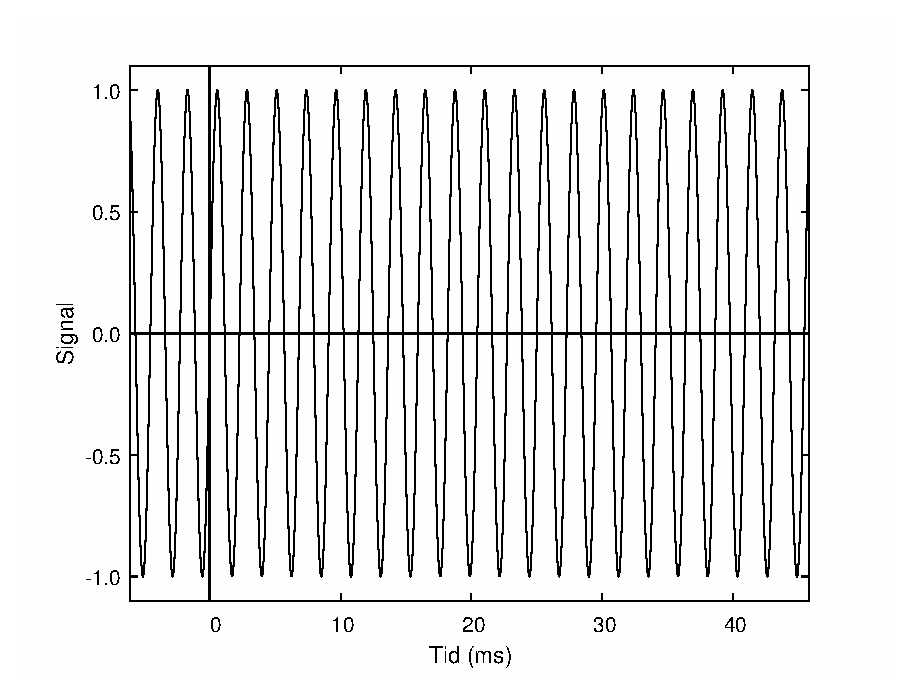
\includegraphics[scale=0.5]{sigconst}
\subcaption{Konstant bærebølge.}
\end{subfigure}
\begin{subfigure}{0.48\textwidth}
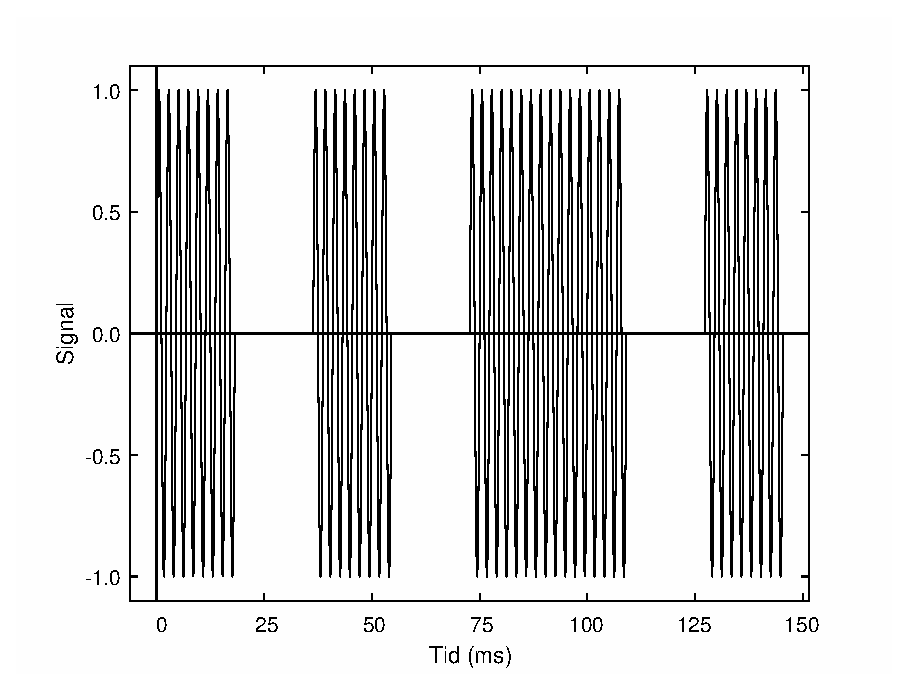
\includegraphics[scale=0.5]{sigask}
\subcaption{Bærebølge moduleret med informationsbit.}
\end{subfigure}
\begin{subfigure}{0.48\textwidth}
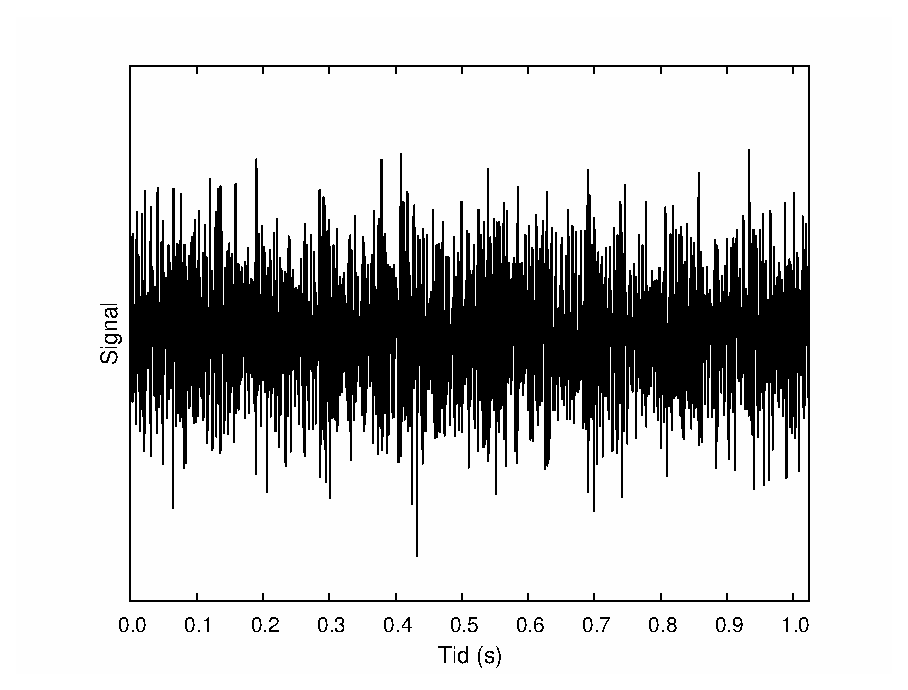
\includegraphics[scale=0.5]{sigrand1}
\subcaption{Udsnit på 1 sek.}
\end{subfigure}
\begin{subfigure}{0.48\textwidth}
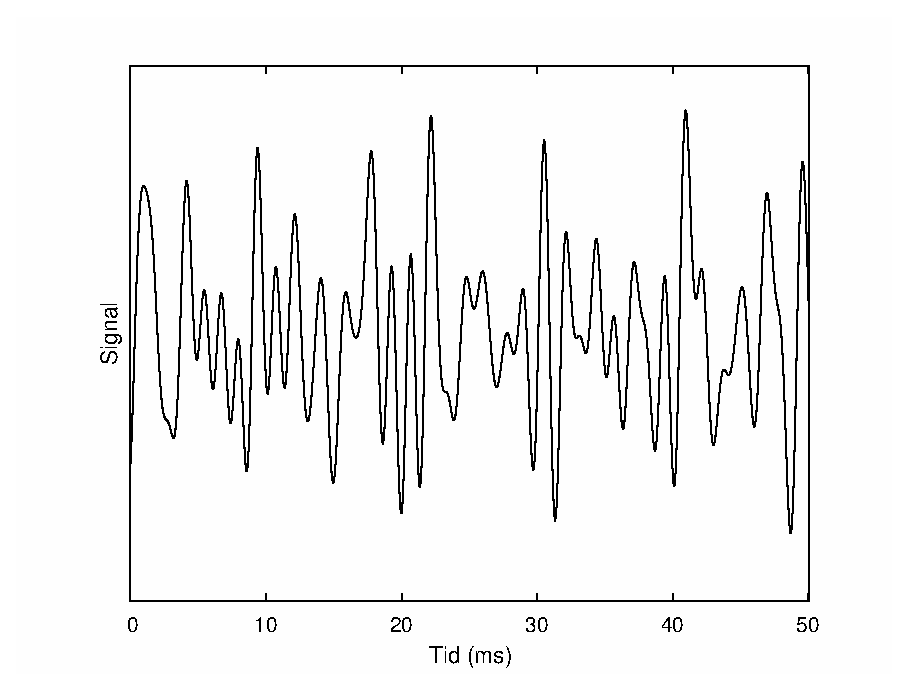
\includegraphics[scale=0.5]{sigrand2}
\subcaption{Udsnit på ca. 50 ms.}
\end{subfigure}
\caption{\label{fig:sig1}Eksempler på signaler.}
\end{figure}

I et virkeligt kommunikationssystem kan brugernes information, og dermed de transmitterede signaler, ikke bestemmes på forhånd, dvs. signalerne er i en vis forstand tilfældige, som i figur~\ref{fig:sig1}c)-d). I dette tilfælde kaldes signalerne for stokastiske signaler, og beregninger på disse kræver kendskab til metoder fra sandsynlighedsregning, så for at forsimple betragtningerne i denne undervisningsnote er det derfor valgt, at der kun betragtes \emph{deterministiske} signaler, dvs. signaler hvor informationsindholdet i princippet er kendt på forhånd. 

\section{Periodiske signaler}
En simpel type af kontinuerte og deterministiske signaler er \emph{periodiske} signaler. Et periodisk signal er defineret ved, at det "gentager" sig selv efter et tidsrum, kaldet signalets \emph{periode}. Dvs. hvis signalet beskrives ved en funktion af tid, dvs. $v(t)$, vil der for et periodisk signal gælde, at
\begin{equation}\label{eq:periodic}
v(t) = v(t + P)
\end{equation}
hvor $P$ så er signalet periode. Bemærk, at hvis $v(t) = v(t+P)$ vil det også gælde for $v(t)=v(t+2P)=v(t+3P)=\ldots=v(t+k\cdot{}P)$ (for $k\in{}\mathbb{N}$). Derfor defineres (grund-)perioden, kaldet $P$, for signalet, som den mindste værdi af $P$, hvor ligning~\ref{eq:periodic} er opfyldt.

Bemærk at man har fuld viden om et signals værdi til alle tidspunkter, hvis man bare kender signalet inden for en enkelt periode, ofte enten tidsintervallet $t\in\left[0;P\right[$ eller tidsintervallet $t\in\left[\frac{-P}{2};\frac{+P}{2}\right[$, da værdien af signalet til alle andre tidspunkter kan udregnes ud fra ligning~(\ref{eq:periodic}).

I stedet for at udtrykke signalet ved dets periode er det også normalt at benytte signalets \emph{frekvens}, $f$, der udtrykker, hvor mange gange pr. sekund, at signalet gentager sig selv. Dvs. signalets frekvens er relateret til signalets periode ved relationen         
\begin{equation}
f=\frac{1}{P}\quad\Leftrightarrow\quad{}P=\frac{1}{f}
\end{equation}

\noindent{}Da $P$ udtrykker et tidsinterval vil enheden være sekunder (s). For frekvensen vil enheden være $s^{-1}$ (fordi det er antallet af gange \emph{per sekund}, at signalet gentager sig), men traditionelt bruges i stedet enheden hertz (forkortet Hz). Det er dog helt ækvivalent at udtrykke, at et signal har en frekvens på $f=100\textrm{ Hz}$ som $f=100\textrm{ s}^{-1}$. Med enheden hertz er det også nemmere at udtrykke høje frekvenser ved at sætte et præfiks foran, som f.eks. kHz, MHz, GHz, osv.

Et simpelt eksempel på et periodisk signal er et cosinus signal, som illustreret i figur~\ref{fig:cos}, hvor signalet i dette eksempel har en periode på $P=1\textrm{ ms}$, svarende til en grundfrekvens på $f_0=1000\textrm{ Hz}$.
\begin{figure}[htbp]
\centering
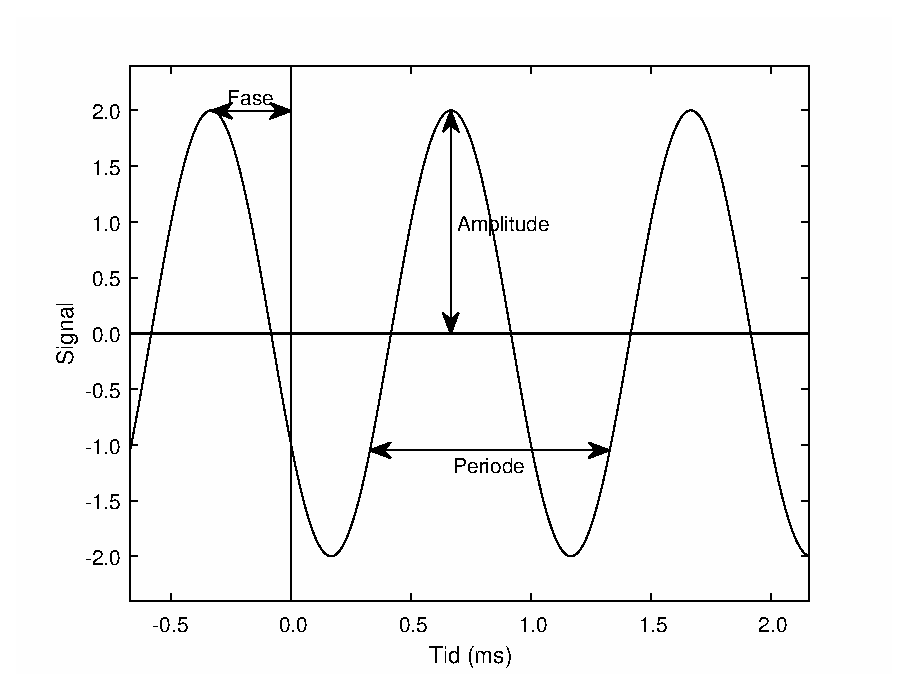
\includegraphics[scale=0.7]{cossignal}
\caption{\label{fig:cos}Cosinus signal.}
\end{figure}

\noindent{}Signalet i figur~\ref{fig:cos} kan i tidsdomænet beskrives ved udtrykket
\begin{equation}\label{eq:cossignal}
v(t) = A\cdot{}\cos\left(2\pi\cdot\frac{t}{P}+\phi\right) = A\cdot{}\cos\left(2\pi\cdot{}f\cdot{}t+\phi\right)
\end{equation}
\noindent{}hvor $A$ er signalets amplitude, $P$ er signalets periode, $f$ er signalets frekvens samt $\phi$ er signalets fase. Som det ses på figuren udtrykker fasen, hvor meget cosinus-kurven er ''forskubbet'' i forhold til kurven $A\cdot{}\cos\left(2\pi\cdot{}f\cdot{}t\right)$. Ved en positiv værdi af fasen $\phi$ vil det toppunkt for cos()-kurven, som ellers vil ligge ved $t=0$, blive forskudt mod negative $t$-værdier (dvs. mod venstre i grafen), mens det modsatte vil være tilfældet ved en negativ $\phi$ værdi.

Det ses, at ligning~(\ref{eq:cossignal}) udtrykker et periodisk signal med perioden $P$, da
\begin{align*}
v(t + P) &= A\cdot{}\cos\left(2\pi\frac{(t+P)}{P}+\phi\right) \nonumber\\
         &= A\cdot{}\cos\left(2\pi\frac{t}{P}+2\pi\frac{P}{P}+\phi\right) \nonumber\\
         &= A\cdot{}\cos\left(2\pi\frac{t}{P}+\phi+2\pi\right) \nonumber\\
         &= A\cdot{}\cos\left(2\pi\frac{t}{P}+\phi\right) \nonumber\\
         &= v(t)
\end{align*}
\noindent{}hvor det undervejs er udnyttet, at $\cos(x+2\pi{})=\cos(x)$.

Signalet illustreret i figur~\ref{fig:cos} består af kun én frekvens. Et mere generelt periodisk signal kan f.eks. konstrueres ud fra et antal forskellige frekvenser, hvor der i det generelle tilfælde ved hver frekvens kan være forskellig amplitude og fase, dvs. signalet kan beskrives som
\begin{alignat}{3}\label{eq:periodic2}
& v(t) && =\ && C_{1}\cdot{}\cos(2\pi\cdot{}f_{1}\cdot{}t+\phi_{1}) + C_{2}\cdot{}\cos(2\pi\cdot{}f_{2}\cdot{}t+\phi_{2}) + \nonumber\\ 
& &&\ && C_{3}\cdot{}\cos(2\pi\cdot{}f_{3}\cdot{}t+\phi_{3}) + \ldots\nonumber \\
& && =\ && \sum_{k} C_{k}\cdot{}\cos(2\pi\cdot{}f_{k}\cdot{}t+\phi_{k})
\end{alignat}

Som eksempel viser figur~\ref{fig:phaseillustration} to perioder af et periodisk signal, hvor der indgår to frekvenser, $f_{1}=100\textrm{ Hz}$ og $f_{2}=200\textrm{ Hz}$; begge med amplituden lig 1, dvs. $C_{1}=C_{2}=1$. Det ene signals fase er blot $\phi_{1}=0$ og det andet signals fase er hhv. $\phi_{2}=0,\frac{\pi}{4},\frac{\pi}{3},\frac{\pi}{2},\frac{3\pi}{4}$ og $\pi$ for at illustrere, hvordan forskelle i signalernes faser kan ændre udseendet af det periodiske signal.
\begin{figure}[htbp]
\centering
\begin{subfigure}{0.48\textwidth}
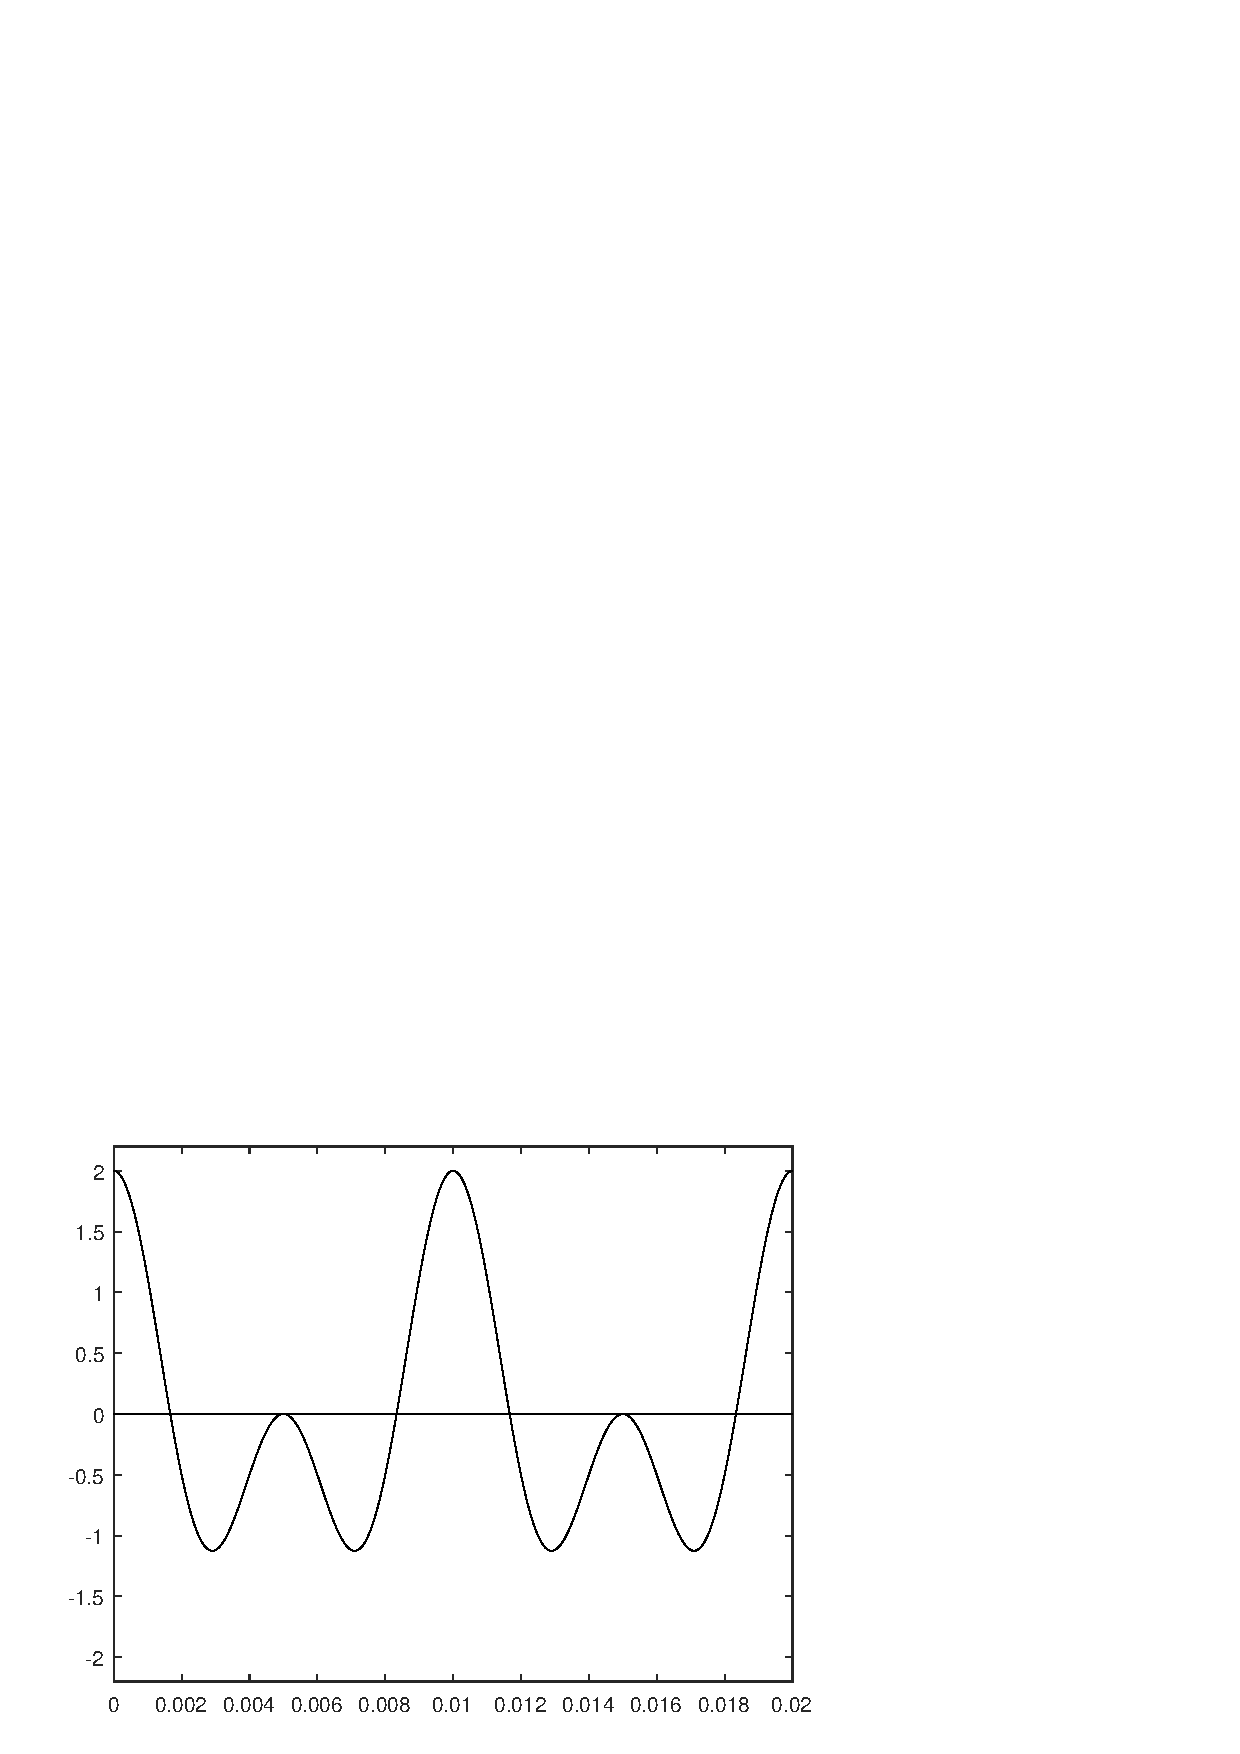
\includegraphics[scale=0.5]{phase_000}
\subcaption{$\phi_{2}=0$.}
\end{subfigure}
\begin{subfigure}{0.48\textwidth}
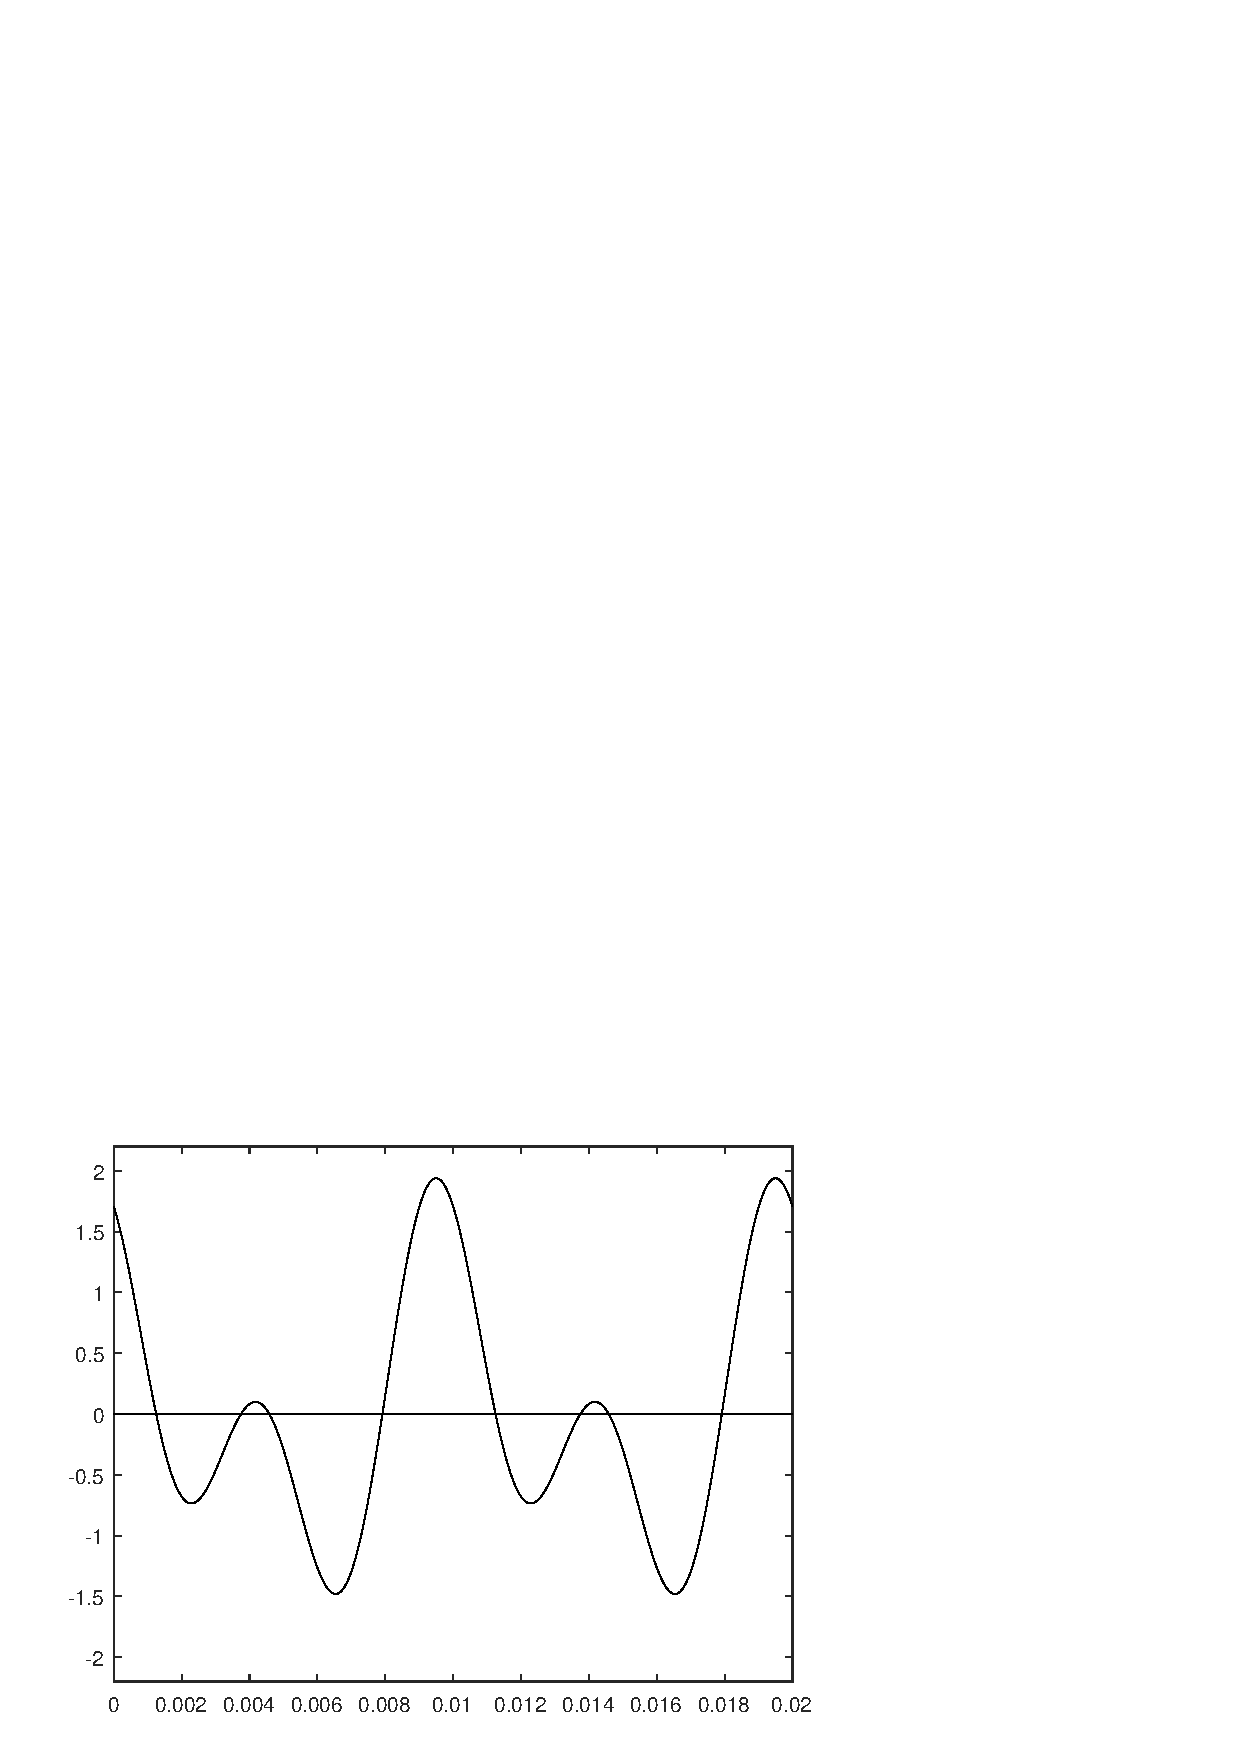
\includegraphics[scale=0.5]{phase_045}
\subcaption{$\phi_{2}=\frac{\pi}{4}$.}
\end{subfigure}
\begin{subfigure}{0.48\textwidth}
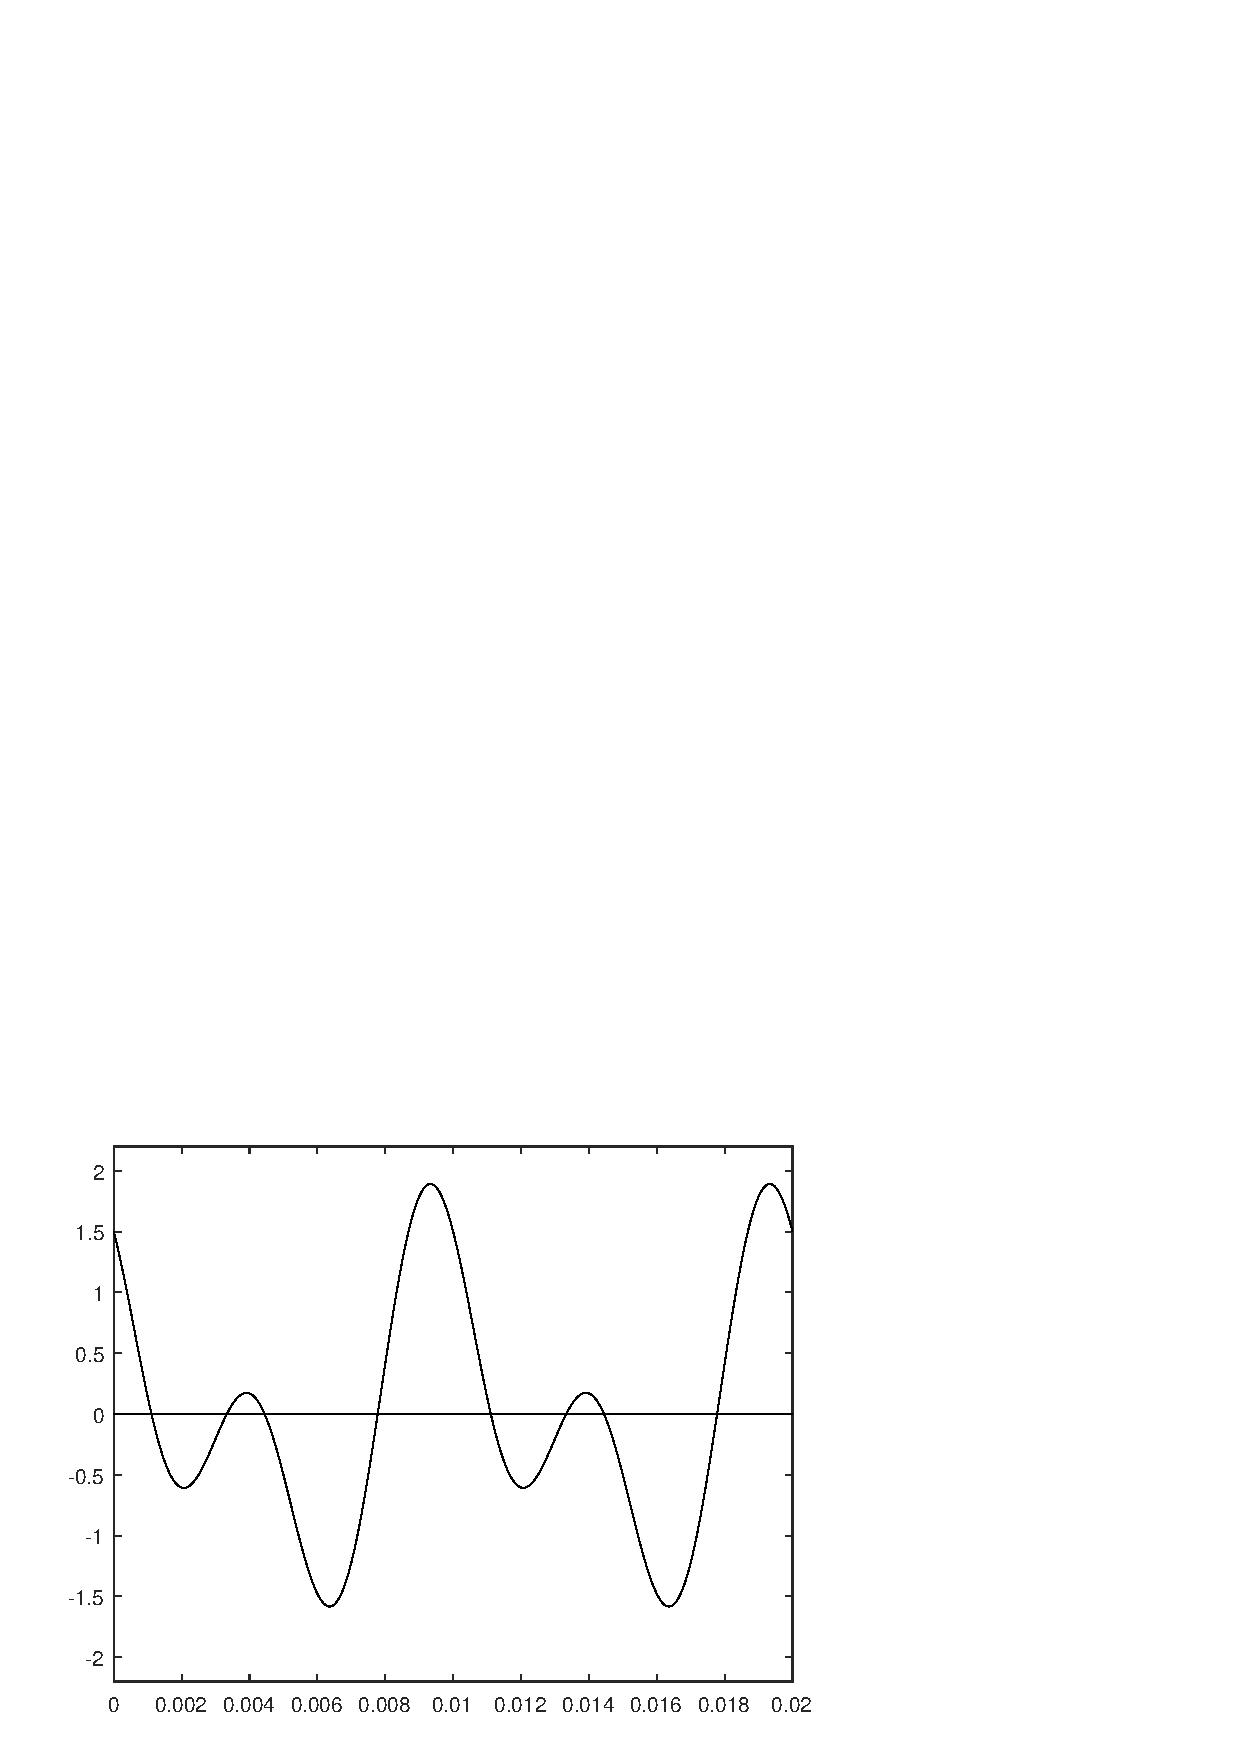
\includegraphics[scale=0.5]{phase_060}
\subcaption{$\phi_{2}=\frac{\pi}{3}$.}
\end{subfigure}
\begin{subfigure}{0.48\textwidth}
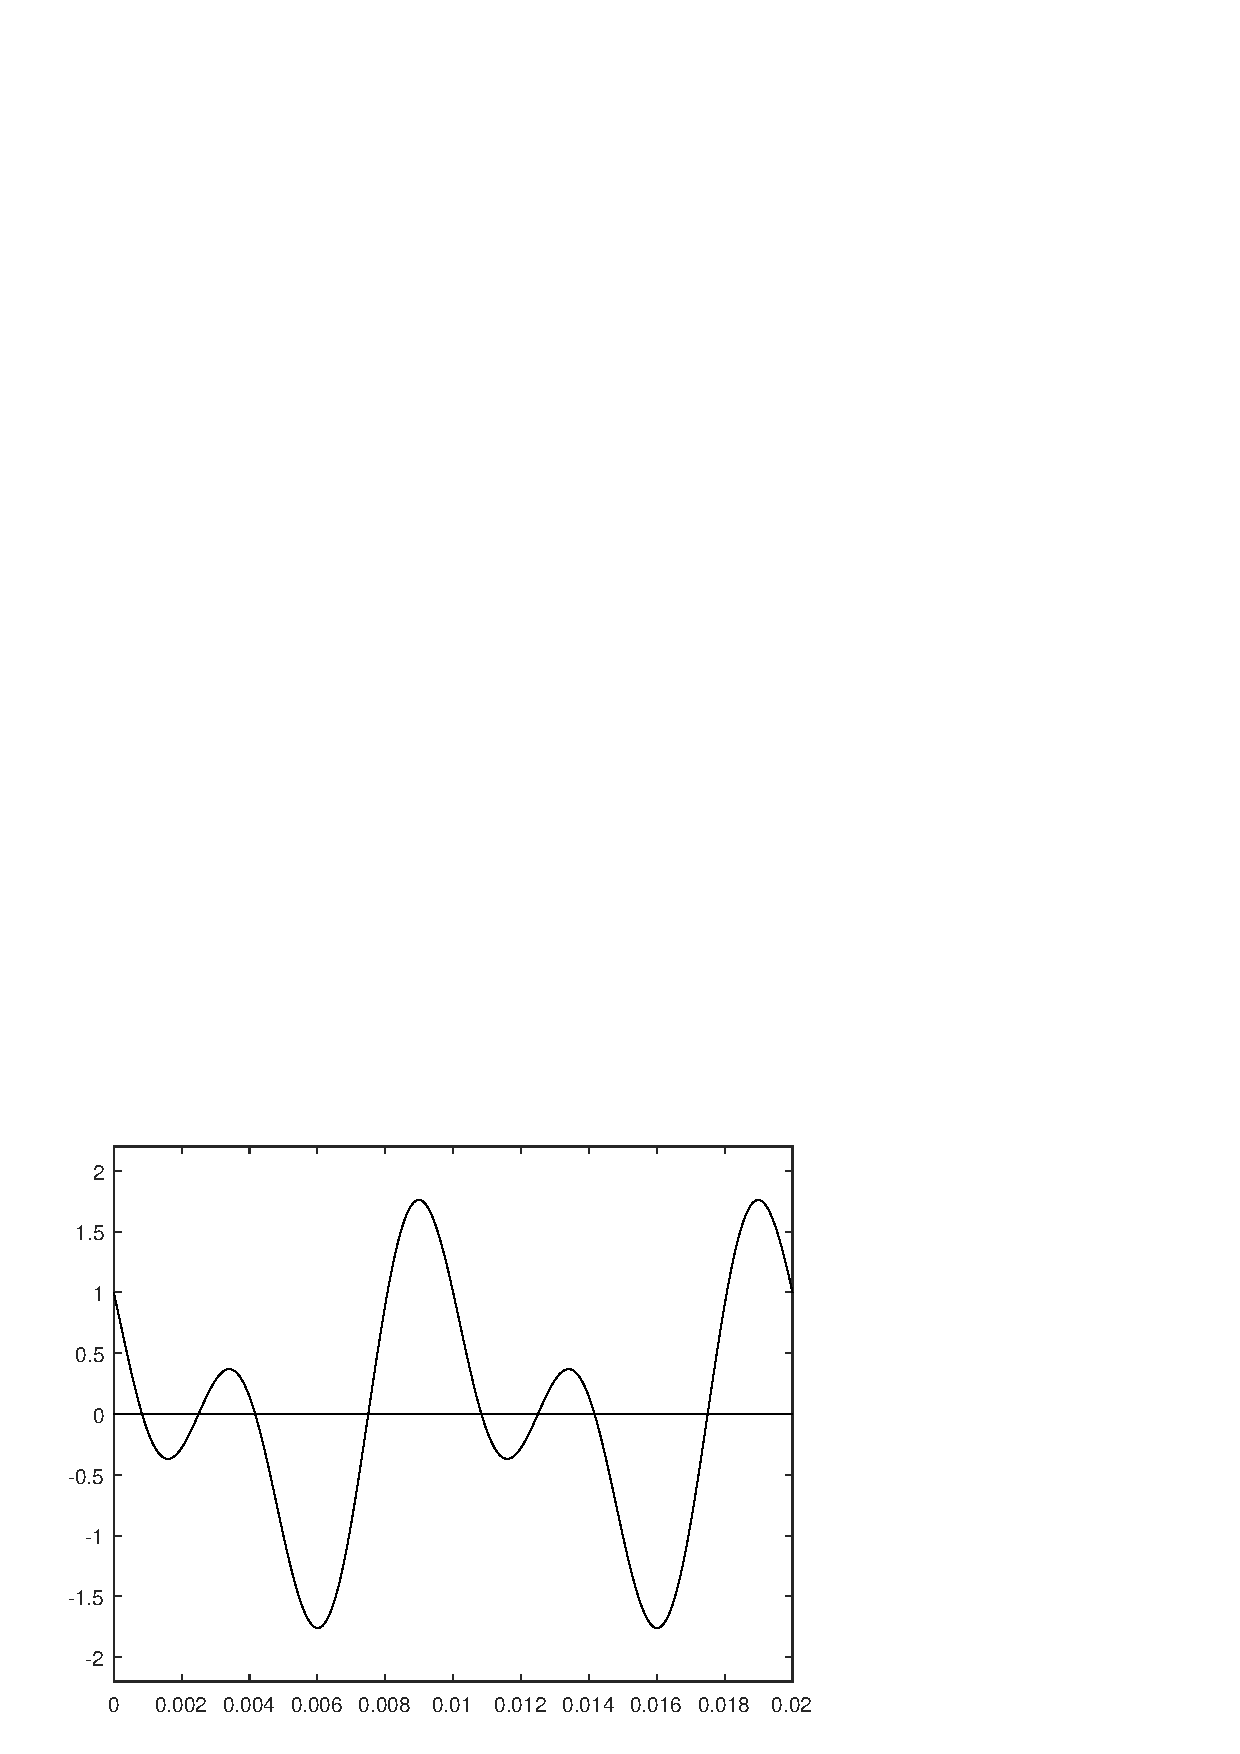
\includegraphics[scale=0.5]{phase_090}
\subcaption{$\phi_{2}=\frac{\pi}{2}$.}
\end{subfigure}
\begin{subfigure}{0.48\textwidth}
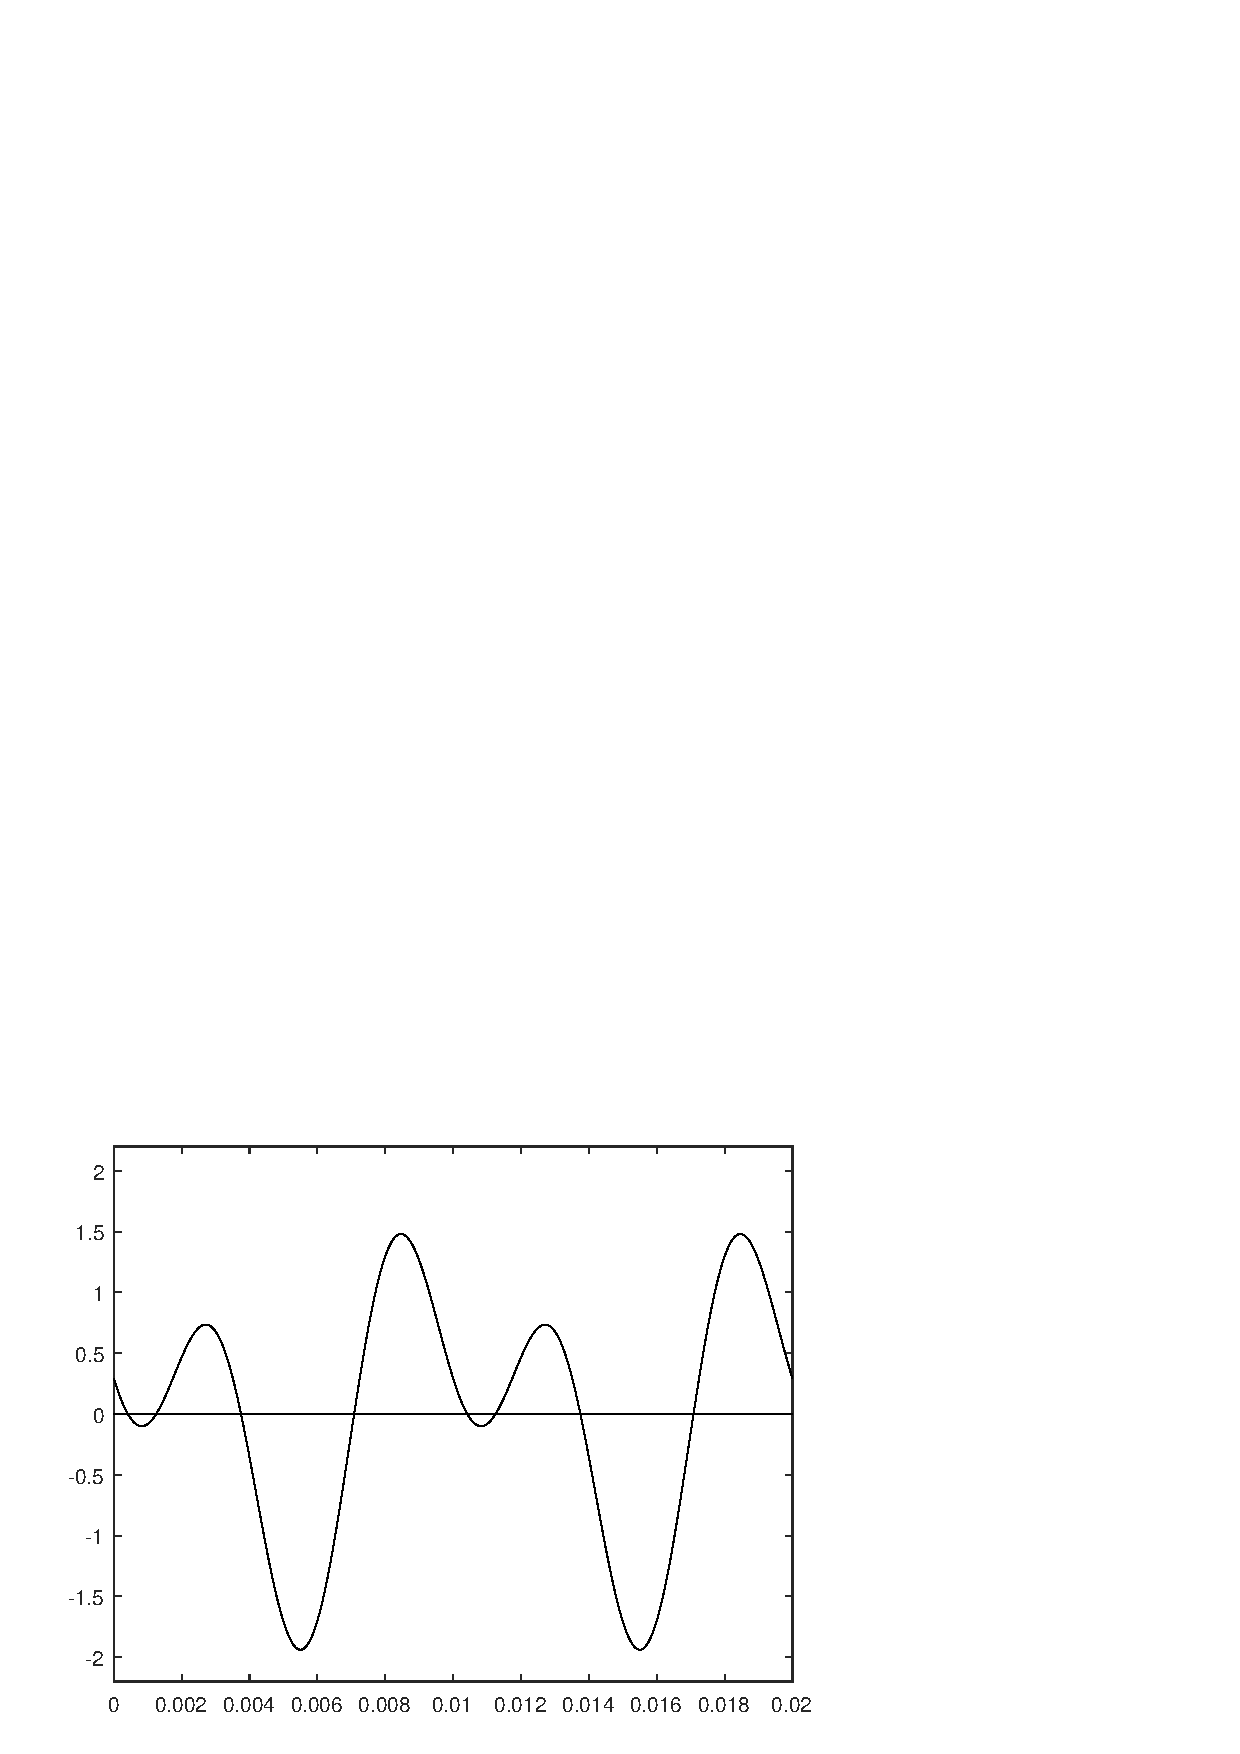
\includegraphics[scale=0.5]{phase_135}
\subcaption{$\phi_{2}=\frac{3\pi}{4}$.}
\end{subfigure}
\begin{subfigure}{0.48\textwidth}
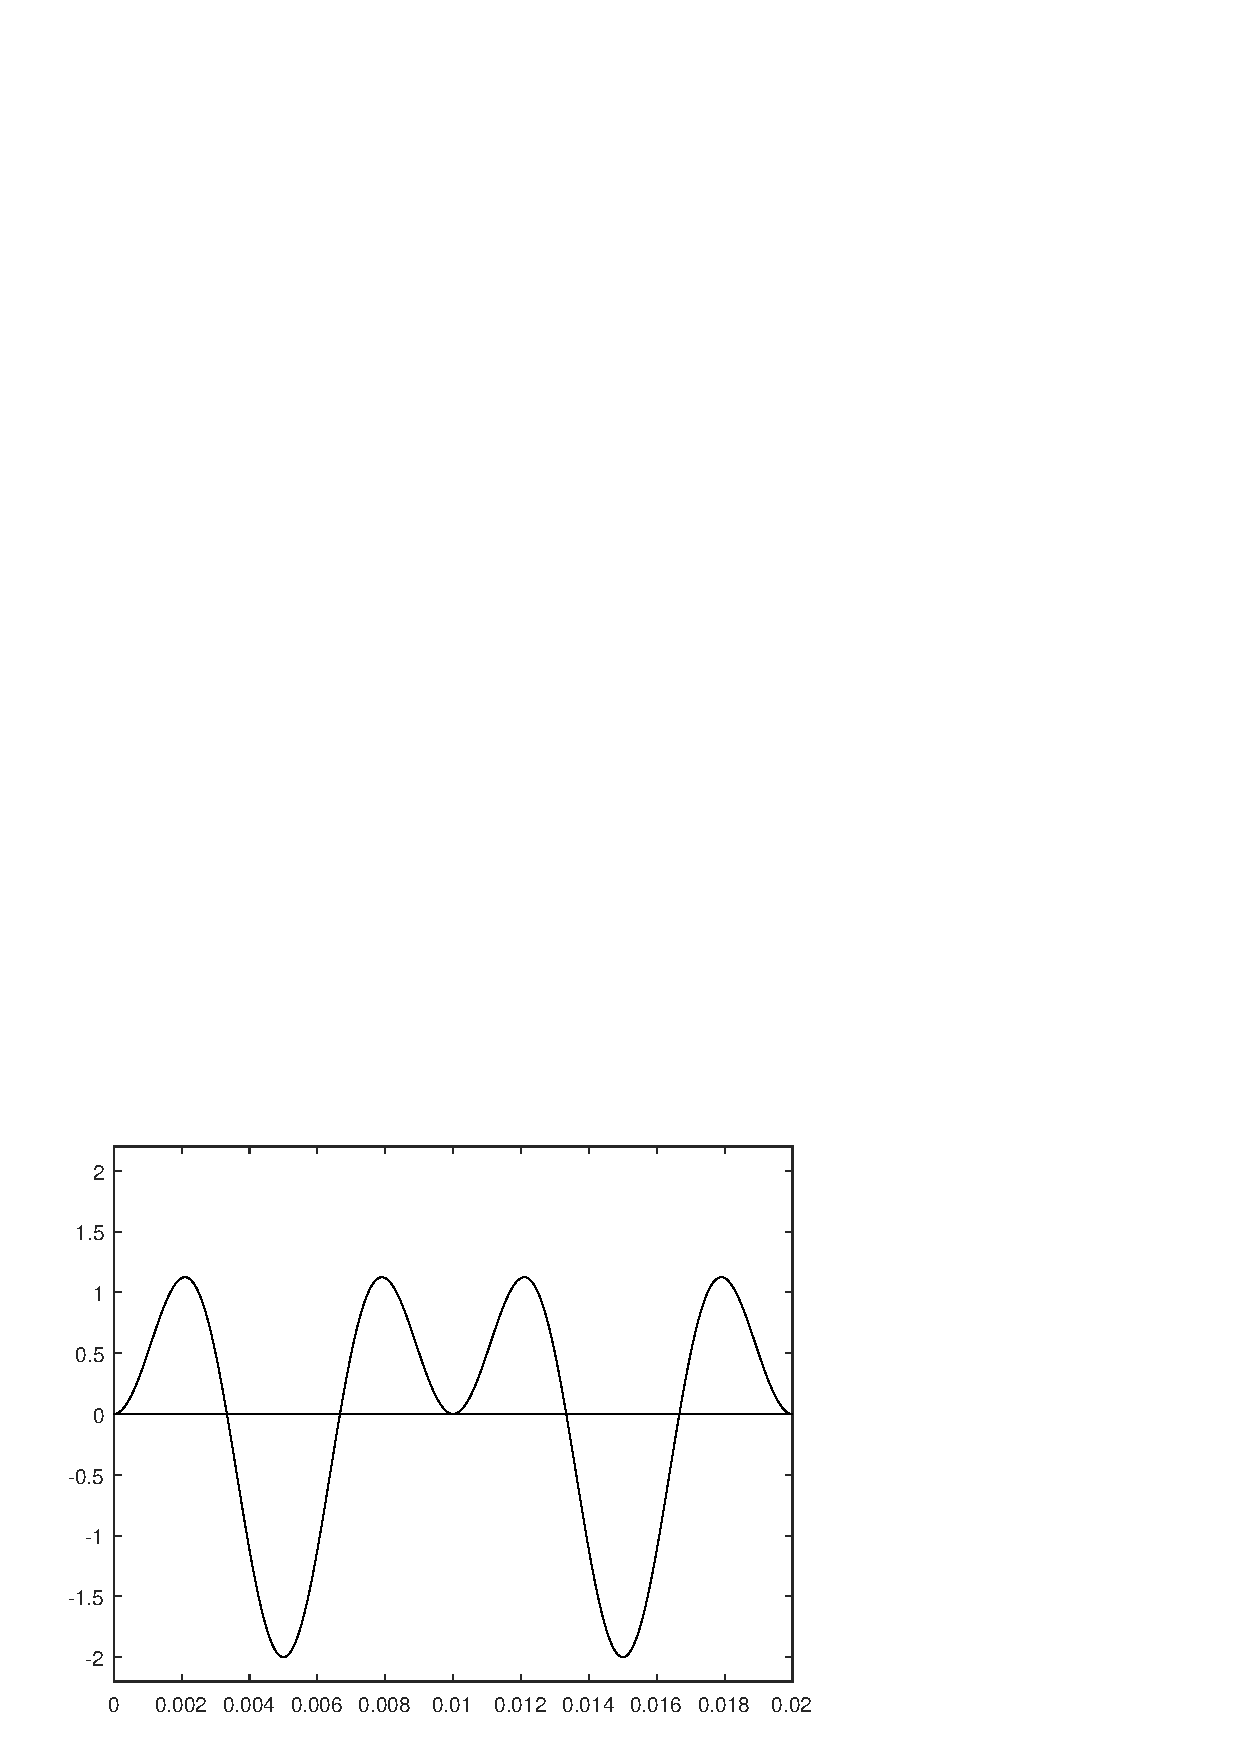
\includegraphics[scale=0.5]{phase_180}
\subcaption{$\phi_{2}=\pi$.}
\end{subfigure}
\caption{\label{fig:phaseillustration}Periodisk signal med to frekvenser og forskellige faser.}
\end{figure}

Perioden for det vilkårlige periodiske signal i formel~(\ref{eq:periodic2}) vil afhænge af perioderne af de enkelte frekvensbidrag, ved at være det \emph{mindste} tidsinterval, som er et multiplum af \emph{samtlige} de enkelte frekvensbidrags perioder, dvs. perioden for det vilkårlige periodiske signal vil være den mindste værdi der opfylder relationen (hvor $l_{i}\in\mathbb{N}$)
\begin{equation}
P=l_{1}\cdot\frac{1}{f_{1}}=l_{2}\cdot\frac{1}{f_{2}}=l_{3}\cdot\frac{1}{f_{3}}=\ldots
\end{equation}
\noindent{}hvilket kan skrives som
\begin{equation}
P=\textrm{lcm}\left(\frac{1}{f_{1}}, \frac{1}{f_{2}}, \frac{1}{f_{3}}, \ldots\right)
\end{equation}
hvor funktionen $\textrm{lcm}(\ldots)$ returnerer det mindste fælles multiplum (på engelsk: \emph{least common multiple}) af funktionens argumenter. Grundfrekvensen, $f_{0}$, for det vilkårlige periodiske signal vil så være $1/P$, hvilket vil være det samme som
\begin{equation}
f_{0}=\gcd\left(f_{1},f_{2},f_{3},\ldots\right)
\end{equation}
hvor funktionen $\gcd(\ldots)$ returnerer det største tal, der går op i alle funktionens argumenter, dvs. den største fælles divisor (på engelsk: \emph{greatest common divisor}) for funktionens argumenter. Bemærk at perioden for det vilkårlige periodiske signal sagtens kan være længere end den længste af perioderne for de enkelte frekvensbidrag, hvilket er det samme som at grundfrekvensen godt kan være mindre end den laveste frekvens der indgår i udtrykket i ligning~(\ref{eq:periodic2}).

\vspace{\baselineskip}\noindent{}\textbf{Eksempel}: Hvis et signal består af to frekvenser, $f_1=200\textrm{ Hz}$ og $f_2=300\textrm{ Hz}$, svarende til perioderne $P_1=5\textrm{ ms}$ og $P_2=3\frac{1}{3}\textrm{ ms}$, vil perioden for det kombinerede signal være $P=10\textrm{ ms}$, fordi tidsintervallet $10\textrm{ ms}$ er det mindste tidsinterval, som både $P_1$ og $P_2$ går op i. Grundfrekvensen er derfor $f_0=1/P=100\textrm{ Hz}$.\vspace{\baselineskip}

For at et vilkårligt periodisk signal af samme form som i ligning~(\ref{eq:periodic2}) skal have en endelig periode, skal det gælde, at forholdet mellem to \emph{vilkårlige} af signalets frekvenser skal være et rationelt tal. Dette er blot det samme som, at alle frekvenserne i signalet skal være et multiplum af den samme grundfrekvens, $f_0$, dvs. ($m_{i}\in\mathbb{N}$)
\begin{equation}
f_{1}=m_{1}\cdot{}f_{0},\quad{}f_{2}=m_{2}\cdot{}f_{0},\quad{}f_{3}=m_{3}\cdot{}f_{0},\ldots{}
\end{equation}

\noindent{}I dette tilfælde kan signalet i formel~(\ref{eq:periodic2}) skrives som:
\begin{alignat}{3}
& v(t) && =\  && C_{1}\cdot{}\cos(2\pi\cdot{}k_{1}\cdot{}f_{0}\cdot{}t+\phi_{1}) + C_{2}\cdot{}\cos(2\pi\cdot{}k_{2}\cdot{}f_{0}\cdot{}t+\phi_{2}) + \nonumber\\
& && \;  && C_{3}\cdot{}\cos(2\pi\cdot{}k_{3}\cdot{}f_{0}\cdot{}t+\phi_{3}) + \ldots \nonumber\\
& && =\  && \sum_{k} C_{k}\cdot{}\cos(2\pi\cdot{}m_{k}\cdot{}f_{0}\cdot{}t+\phi_{k})\label{eq:periodic3}
\end{alignat}

\noindent{}Bemærk at der i formel~(\ref{eq:periodic3}) summeres over alle de frekvenser, der indgår i signalet. Dette kan generaliseres til en uendelig sum over alle multipla af grundfrekvensen, $f_0$. For de frekvenser, der ikke indgår i signalet, vil de tilhørende $C_k$-værdier blot være lig 0. Hvis signalet er dannet ud fra et endeligt antal frekvenser, vil det så blot svare til, at der er en største værdi af $k$, kaldet $k_{max}$, hvor $C_k\ne{}0$, dvs. $C_k = 0$ for $k > k_{max}$. Det generelle periodiske signal kan derfor skrives som
\begin{equation}\label{eq:periodic4}
v(t)=\sum_{k=0}^{\infty} C_{k}\cdot{}\cos(2\pi\cdot{}m_{k}\cdot{}f_{0}\cdot{}t+\phi_{k})
\end{equation}

\noindent{}Bemærk at summen i ligning~(\ref{eq:periodic4}) inkluderer frekvensen $0\cdot{}f_0$, dvs. 0~Hz. Dette repræsenterer et konstant bidrag til signalet (da $\cos(0)=1$), der repræsenterer signalets middelværdi. Figur~\ref{fig:cossignal2} illustrerer betydningen af et konstant bidrag -- begge kurver i figuren har perioden 1~ms, svarende til grundfrekvensen $f_0=1000\textrm{ Hz}$ (alle $\phi_k$-værdier er lig 0). Den fuldt optrukne kurve i figuren viser et signal $C_1=2$ (og alle andre $C_k$-værdier lig 0), mens den stiplede kurve har $C_0=1$, $C_1=2$ (og alle andre $C_k$-værdier lig 0). Som det ses er den stiplede kurve er blevet forskudt med værdien $C_0$ i forhold til kurven med $C_0=0$.
\begin{figure}[htbp]
\centering
\scalebox{0.7}{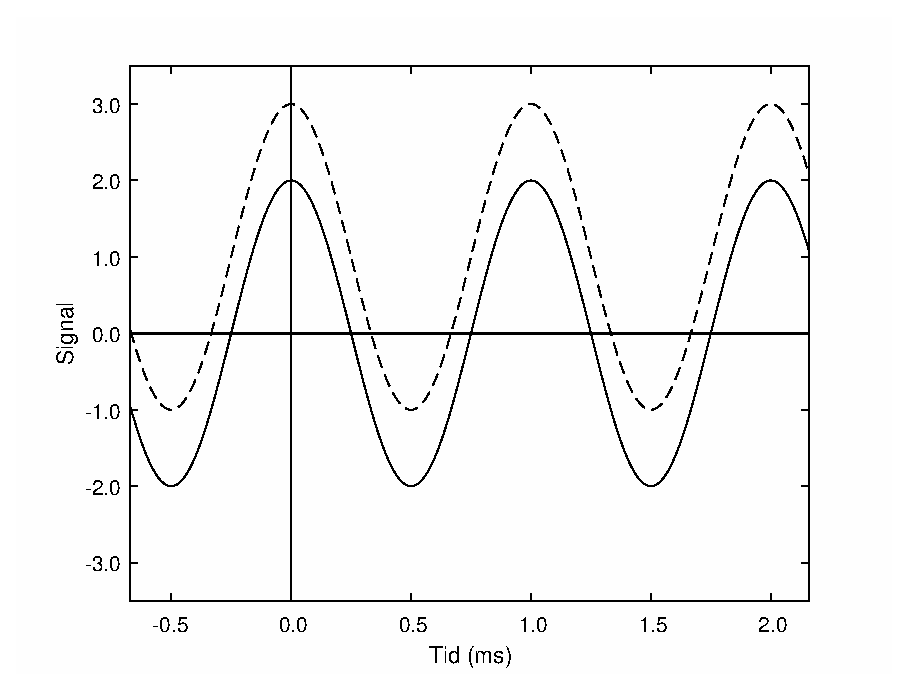
\includegraphics[]{cossignal2}}
\caption{\label{fig:cossignal2}Betydning af konstant bidrag.}
\end{figure}

Man kan også betragte periodiske signaler, som ikke umiddelbart ser ud til at have noget med en sum af et antal $\cos()$-funktioner at gøre. F.eks. viser figur~\ref{fig:squareperiodic} to periodiske signal (med $P=1$ i begge tilfælde). I figur~\ref{fig:squareperiodic}a) fremkommer signalet som en periodisk gentagelse af funktionen $v(t)=t^{2}$ for $-\frac{P}{2}\le{}t<\frac{P}{2}$, og i figur~\ref{fig:squareperiodic}b) er signalet et såkaldt \emph{firkantsignal}, hvor signalet inden for en periode er defineret ved
\begin{equation}
v_{\textrm{firkant}}=
\begin{cases}
-1 & \quad \text{for } -P/2 \leq t < -P/4 \\
+1 & \quad \text{for } -P/4 \leq t < +P/4 \\
-1 & \quad \text{for } +P/4 \leq t < +P/2 \\
\end{cases}
\end{equation}

\begin{figure}[htbp]
\centering
\begin{subfigure}{0.48\textwidth}
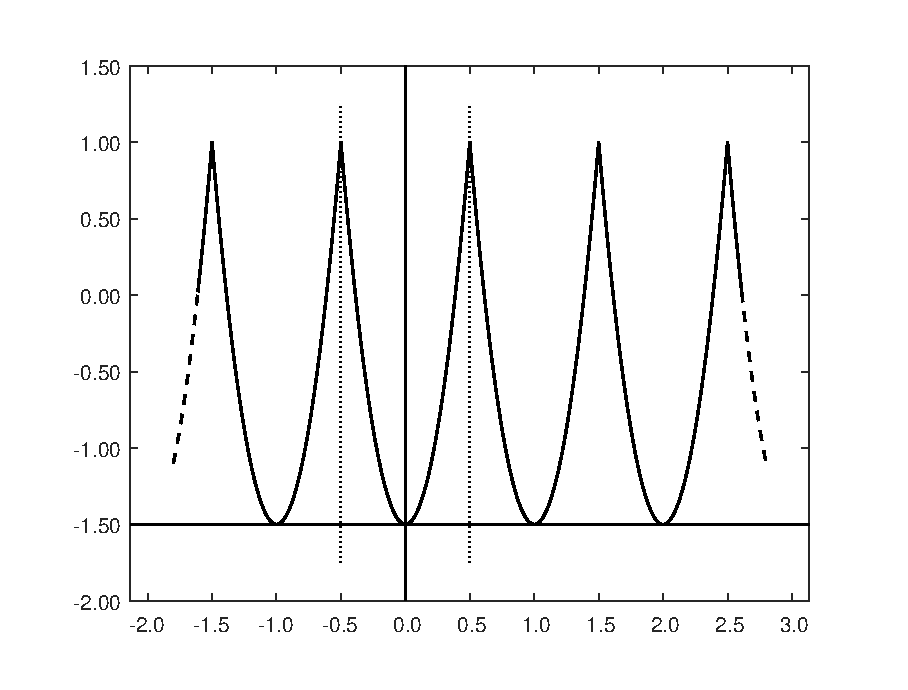
\includegraphics[scale=0.5]{squared1}
\subcaption{Periodisk gentagelse af $v(t)=t^{2}$.}
\end{subfigure}
\begin{subfigure}{0.48\textwidth}
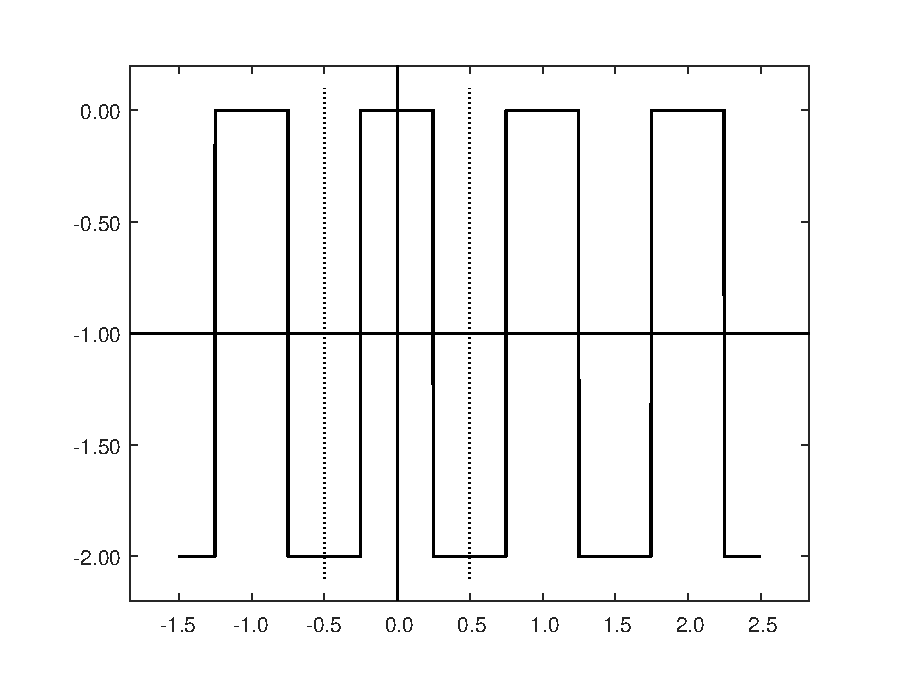
\includegraphics[scale=0.5]{squared2}
\subcaption{Firkantsignal}
\end{subfigure}
\caption{\label{fig:squareperiodic}To forskellige periodiske signaler.}
\end{figure}

Umiddelbart er det nok svært at relatere formeludtrykket i formel~(\ref{eq:periodic4}) med signalerne i figur~\ref{fig:squareperiodic}, men det er faktisk muligt at finde værdier for $C_{k}$ og $\phi_{k}$ i formel~(\ref{eq:periodic4}) der giver signalerne i figur~\ref{fig:squareperiodic}. Helt generelt gælder\footnote{Et matematisk bevis for sætning 1 vil dog ikke blive givet her} nemlig:

\vspace{\baselineskip}\fbox{\parbox{0.9\textwidth}{\textbf{Sætning 1:} Enhver kontinuert periodisk funktion, $v(t)$ med (grund-)perioden $P$ (og dermed grundfrekvensen $f_0$) kan beskrives ved:
\begin{equation}\label{eq:periodic5}
v(t)=\sum_{k=0}^{\infty} C_{k}\cdot\cos(2\pi\cdot{}\frac{k}{P}\cdot{}t+\phi_{k})=\sum_{k=0}^{\infty} C_{k}\cdot\cos(2\pi\cdot{}k\cdot{}f_{0}\cdot{}t+\phi_{k})
\end{equation}
\noindent{}for passende værdier af $C_k$ og $\phi_k$.
}}\vspace{\baselineskip}

Dette betyder endvidere, at hvis man har et vilkårligt periodisk signal kan man -- ved at finde de korrekte $C_k$- og $\phi_k$ værdier -- bestemme, hvor hvilket bidrag der er ved de forskellige frekvenser til det generelle periodiske signal. Jo større $C_k$-værdi, jo større bidrag af frekvensen $k\cdot{}f_0$ er der til det periodiske signal.

Umiddelbart er det nok ikke indlysende fra formel~(\ref{eq:periodic5}), hvordan man -- ud fra et vilkårligt periodisk signal -- skal kunne finde de korrekte $C_k$- og $\phi_k$-værdier, der tilsammen beskriver signalet. Første trin er derfor en omskrivning af formlen, for at "slippe af med" fasebidragene i formlen. Hertil benyttes additionsformlen for $\cos()$:
\begin{equation}
\cos(x+y)=\cos(x)\cdot\cos(y)-\sin(x)\cdot\sin(y)
\end{equation}

\noindent{}Dvs. de enkelte led i summen i formel~(\ref{eq:periodic5}) kan omskrives på flg. måde:
\begin{multline*}
C_{k}\cdot\cos(2\pi\cdot{}k\cdot{}f_{0}\cdot{}t+\phi_{k}) = \\
C_{k}\cdot\left(\cos(2\pi\cdot{}k\cdot{}f_{0}\cdot{}t)\cdot\cos(\phi_{k})-\sin(2\pi\cdot{}k\cdot{}f_{0}\cdot{}t)\cdot\sin(\phi_{k})\right)=\\
C_{k}\cdot\cos(2\pi\cdot{}k\cdot{}f_{0}\cdot{}t)\cdot\cos(\phi_{k})-C_{k}\cdot\sin(2\pi\cdot{}k\cdot{}f_{0}\cdot{}t)\cdot\sin(\phi_{k})
\end{multline*}

\noindent{}Hvis man indfører substitutionerne $A_{k}=C_{k}\cdot\cos(\phi_{k})$ og $B_{k}=-C_{k}\cdot\sin(\phi_{k})$ fås derved, at 
\begin{equation*}
C_{k}\cdot\cos(2\pi\cdot{}k\cdot{}f_{0}\cdot{}t+\phi_{k}) = 
A_{k}\cdot\cos(2\pi\cdot{}k\cdot{}f_{0}\cdot{}t)+B_{k}\cdot\sin(2\pi\cdot{}k\cdot{}f_{0}\cdot{}t)
\end{equation*}

\noindent{}Dvs. sætning 1 kan nu omformuleres til:

\vspace{\baselineskip}\fbox{\parbox{0.9\textwidth}{\textbf{Sætning 2:} Enhver kontinuert periodisk funktion, $v(t)$ med perioden $P$ (og dermed grundfrekvensen $f_0$) kan beskrives ved:
\begin{equation}\label{eq:periodic6}
v(t)=\sum_{k=0}^{\infty} \left\lbrace{}A_{k}\cdot\cos(2\pi\cdot{}k\cdot{}f_{0}\cdot{}t)+B_{k}\cdot\sin(2\pi\cdot{}k\cdot{}f_{0}\cdot{}t)\right\rbrace
\end{equation}
\noindent{}for passende værdier af $A_k$ og $B_k$.
}}\vspace{\baselineskip}

\noindent{}Dvs. et vilkårligt periodisk signal kan beskrives enten ved $v(t)$ eller ved at kende alle $A_{k}$- og $B_{k}$-værdier (eller alternativt: alle $C_k$ og $\phi_k$ værdier). Det ses også ud fra formel~(\ref{eq:periodic6}) at funktionerne $\cos(2\pi\cdot{}k\cdot{}f_{0}\cdot{}t)$ og $\sin(2\pi\cdot{}k\cdot{}f_{0}\cdot{}t)$ er en slags ''byggeklodser'', da de sammen med $A_{k}$- og $B_{k}$-værdierne er med til at ''opbygge'' det periodiske signal.

\section{Ortogonalitet}
En vigtig (i denne sammenhæng) relation mellem funktioner er begrebet \emph{ortogonalitet}, der også kendes fra vektoranalyse. To $n$-dimensionale vektorer siges at være ortogonale, hvis deres prikprodukt er lig 0. For to reelle funktioner, $s_{1}(t)$ og $s_{2}(t)$, ($s_{1},s_{2}:\mathbb{R}\mapsto\mathbb{R}$) gælder noget tilsvarende: To funktioner er \emph{ortogonale} over et interval $\left[ a ; b \right]$, hvis flg. relation er opfyldt:
\begin{equation}\label{eq:ortho}
\int\limits_{a}^{b} s_{1}(t)\cdot{}s_{2}(t)\;{}dt = 0
\end{equation} 

\noindent{}For de reelle funktioner ($\cos()$ og $\sin()$) gælder flg. mht. ortogonalitet\footnote{Formlerne i pkt. 1-3 omkring ortogonalitet anføres her uden udledning/bevis, men de er dog ikke svære at eftervise.}:
\begin{enumerate}
	%
	\item To $\cos()$- og/eller $\sin()$-funktioner med \emph{forskellige} frekvenser (der dog begge er et multiplum af samme grundfrekvens, $f_0$), er ortogonale over intervallet $\left[ -\frac{1}{2f_0} ; \frac{1}{2f_0} \right]=\left[ -\frac{P}{2} ; \frac{P}{2} \right]$, dvs.:
	\begin{gather} 
	\int\limits_{-\frac{P}{2}}^{\frac{P}{2}}\cos(2\pi\cdot{}k_{1}\cdot{}f_{0}\cdot{}t)\cdot{}\cos(2\pi\cdot{}k_{2}\cdot{}f_{0}\cdot{}t)\;dt = 0\quad{}\textrm{for}\quad{}k_{1}\ne{}k_{2}\\
	\int\limits_{-\frac{P}{2}}^{\frac{P}{2}}\cos(2\pi\cdot{}k_{1}\cdot{}f_{0}\cdot{}t)\cdot{}\sin(2\pi\cdot{}k_{2}\cdot{}f_{0}\cdot{}t)\;dt = 0\quad{}\textrm{for}\quad{}k_{1}\ne{}k_{2}\\
	\int\limits_{-\frac{P}{2}}^{\frac{P}{2}}\sin(2\pi\cdot{}k_{1}\cdot{}f_{0}\cdot{}t)\cdot{}\sin(2\pi\cdot{}k_{2}\cdot{}f_{0}\cdot{}t)\;dt = 0\quad{}\textrm{for}\quad{}k_{1}\ne{}k_{2}
	\end{gather}
	%
	\item En $\cos()$-funktion og en $\sin()$-funktion med samme frekvens, $f_{1}$, er ortogonale over intervallet $\left[ -\frac{P}{2} ; \frac{P}{2} \right]$, dvs.:
	\begin{equation} 
	\int\limits_{-\frac{P}{2}}^{\frac{P}{2}}\cos(2\pi\cdot{}k_{1}\cdot{}f_{1}\cdot{}t)\cdot{}\sin(2\pi\cdot{}k_{1}\cdot{}f_{1}\cdot{}t)\;dt = 0
	\end{equation}
	%
	\item Til gengæld er hverken $\cos()$- eller $\sin()$-funktionerne ortogonale med sig selv. For både $\cos()$- og $\sin()$-funktionerne fås for $k>0$:
	\begin{gather}
	\int\limits_{-\frac{P}{2}}^{\frac{P}{2}}\cos(2\pi\cdot{}k\cdot{}f_{0}\cdot{}t)\cdot{}\cos(2\pi\cdot{}k\cdot{}f_{0}\cdot{}t)\;dt = \frac{P}{2} \\
	\int\limits_{-\frac{P}{2}}^{\frac{P}{2}}\sin(2\pi\cdot{}k\cdot{}f_{0}\cdot{}t)\cdot{}\sin(2\pi\cdot{}k\cdot{}f_{0}\cdot{}t)\;dt = \frac{P}{2}
	\end{gather}
\end{enumerate}

I ovenstående formler er benyttet et symmetrisk tidsinterval $\left[ -\frac{1}{2f_{0}} ; \frac{1}{2f_{0}} \right] = \left[ -\frac{P}{2} ; \frac{P}{2} \right]$ for passende $f_{0}$ og $P$ værdier, men formlerne er gyldige for ethvert interval af længden $P$.

\section{Bestemmelse af $A_k$ og $B_k$}
Med resultaterne omkring ortogonalitet af $\cos()$- og $\sin()$-funktionerne fra forrige afsnit er vi nu i stand til at vise, hvordan $A_k$- og $B_k$-værdierne for et vilkårligt periodisk signal kan bestemmes.

Hvis man multiplicerer et periodisk signal med perioden $P$ (og dermed grundfrekvensen $f_0$) med $\cos(2\pi\cdot{}k_{1}\cdot{}f_{0}\cdot{}t)$ (for $k_1>0$) og integrerer over intervallet $\left[ -\frac{P}{2} ; \frac{P}{2} \right]$ fås\footnote{I beviset er anvendt omskrivningen $\int\limits_{a}^b\left(\sum\limits_{k=0}^{\infty}f_{k}(t)\right)dt=\sum\limits_{k=0}^{\infty}\left(\int\limits_{a}^{b}f_{k}(t)dt\right)$, der dog kun gælder, hvis den uendelige sum er \emph{konvergent} - dette er tilfældet her, men beviset er dog udeladt.}:

\begin{gather}
\int\limits_{-\frac{P}{2}}^{\frac{P}{2}}v(t)\cdot\cos(2\pi\cdot{}k_{1}\cdot{}f_{0}\cdot{}t)\;dt = \nonumber\\
%
\int\limits_{-\frac{P}{2}}^{\frac{P}{2}}\Bigg\lbrace\sum_{k=0}^{\infty} \big\lbrace{}A_{k}\cdot\cos(2\pi\cdot{}k\cdot{}f_{0}\cdot{}t)+B_{k}\cdot\sin(2\pi\cdot{}k\cdot{}f_{0}\cdot{}t)\big\rbrace\Bigg\rbrace\cdot\cos(2\pi\cdot{}k_{1}\cdot{}f_{0}\cdot{}t)\;dt\;=\nonumber\\
%
\begin{split}
\int\limits_{-\frac{P}{2}}^{\frac{P}{2}}\Bigg\lbrace\sum_{k=0}^{\infty} \big\lbrace&A_{k}\cdot\cos(2\pi\cdot{}k\cdot{}f_{0}\cdot{}t)\cdot\cos(2\pi\cdot{}k_{1}\cdot{}f_{0}\cdot{}t)+\\
&B_{k}\cdot\sin(2\pi\cdot{}k\cdot{}f_{0}\cdot{}t)\cdot\cos(2\pi\cdot{}k_{1}\cdot{}f_{0}\cdot{}t)\big\rbrace\Bigg\rbrace\;dt\;=
\end{split}\nonumber\\
%
\begin{split}
\sum_{k=0}^{\infty}\Bigg\lbrace\int\limits_{-\frac{P}{2}}^{\frac{P}{2}}\Big\lbrace{}&A_{k}\cdot\cos(2\pi\cdot{}k\cdot{}f_{0}\cdot{}t)\cdot\cos(2\pi\cdot{}k_{1}\cdot{}f_{0}\cdot{}t)+\\
&{}B_{k}\cdot\sin(2\pi\cdot{}k\cdot{}f_{0}\cdot{}t)\cdot\cos(2\pi\cdot{}k_{1}\cdot{}f_{0}\cdot{}t)\Big\rbrace\;dt\Bigg\rbrace{}=
\end{split}\nonumber\\
%
\begin{split}
\sum_{k=0}^{\infty}\Bigg\lbrace
&\int\limits_{-\frac{P}{2}}^{\frac{P}{2}}A_{k}\cdot\cos(2\pi\cdot{}k\cdot{}f_{0}\cdot{}t)\cdot\cos(2\pi\cdot{}k_{1}\cdot{}f_{0}\cdot{}t)\;dt + \\
&\int\limits_{-\frac{P}{2}}^{\frac{P}{2}}B_{k}\cdot\sin(2\pi\cdot{}k\cdot{}f_{0}\cdot{}t)\cdot\cos(2\pi\cdot{}k_{1}\cdot{}f_{0}\cdot{}t)\;dt
\Bigg\rbrace{}=
\end{split}\nonumber\\
%
\begin{split}
\sum_{k=0}^{\infty}\Bigg\lbrace
&A_{k}\cdot\int\limits_{-\frac{P}{2}}^{\frac{P}{2}}\cos(2\pi\cdot{}k\cdot{}f_{0}\cdot{}t)\cdot\cos(2\pi\cdot{}k_{1}\cdot{}f_{0}\cdot{}t)\;dt + \\
&B_{k}\cdot\int\limits_{-\frac{P}{2}}^{\frac{P}{2}}\sin(2\pi\cdot{}k\cdot{}f_{0}\cdot{}t)\cdot\cos(2\pi\cdot{}k_{1}\cdot{}f_{0}\cdot{}t)\;dt
\Bigg\rbrace
\end{split}
\end{gather}

\noindent{}Fra formlerne omkring ortogonalitet ses, at begge integraler i den sidste linje er lig 0 for $k\ne{}k_{1}$, og at det 2. integrale er endvidere også lig 0 for $k=k_1$, hvorfor den den uendelige sum reduceres til
\begin{equation}
A_{k_1}\cdot\int\limits_{-\frac{P}{2}}^{\frac{P}{2}}\cos(2\pi\cdot{}k_{1}\cdot{}f_{0}\cdot{}t)\cdot\cos(2\pi\cdot{}k_{1}\cdot{}f_{0}\cdot{}t)\;dt = A_{k_1}\cdot\frac{P}{2}
\end{equation}

\noindent{}Herved fås:
\begin{equation}
\int\limits_{-\frac{P}{2}}^{\frac{P}{2}}v(t)\cdot\cos(2\pi\cdot{}k_{1}\cdot{}f_{0}\cdot{}t)\;dt = A_{k_1}\cdot\frac{P}{2}
\end{equation}
dvs.
\begin{equation}
A_{k}=\frac{2}{P}\cdot\int\limits_{-\frac{P}{2}}^{\frac{P}{2}}v(t)\cdot\cos(2\pi\cdot{}k\cdot{}f_{0}\cdot{}t)\;dt\label{eq:akoeff}
\end{equation}

\noindent{}På tilsvarende måde kan man multiplicerer det periodiske signal med $\sin(2\pi\cdot{}k_{1}\cdot{}f_{0}\cdot{}t)$ (igen for $k_1>0$) og integrerer over intervallet $\left[ -\frac{P}{2} ; \frac{P}{2} \right]$. Herved fås på samme måde (mellemregningerne er udeladt):
\begin{equation}
B_{k}=\frac{2}{P}\cdot\int\limits_{-\frac{P}{2}}^{\frac{P}{2}}v(t)\cdot\sin(2\pi\cdot{}k\cdot{}f_{0}\cdot{}t)\;dt\label{eq:bkoeff}
\end{equation}

\noindent{}Endelig fås for $k_1=0$, at
\begin{gather}
%
\int\limits_{-\frac{P}{2}}^{\frac{P}{2}}v(t)\cdot\cos(2\pi\cdot{}0\cdot{}f_{0}\cdot{}t)\;dt = \int\limits_{-\frac{P}{2}}^{\frac{P}{2}}v(t)\;dt =\nonumber\\
%
\int\limits_{-\frac{P}{2}}^{\frac{P}{2}}\sum_{k=0}^{\infty} \big\lbrace{}A_{k}\cdot\cos(2\pi\cdot{}k\cdot{}f_{0}\cdot{}t)+B_{k}\cdot\sin(2\pi\cdot{}k\cdot{}f_{0}\cdot{}t)\big\rbrace\;dt\;=\nonumber\\
%
\sum_{k=0}^{\infty}\Bigg\lbrace\int\limits_{-\frac{P}{2}}^{\frac{P}{2}}\big\lbrace{}A_{k}\cdot\cos(2\pi\cdot{}k\cdot{}f_{0}\cdot{}t)+B_{k}\cdot\sin(2\pi\cdot{}k\cdot{}f_{0}\cdot{}t)\big\rbrace\;dt\Bigg\rbrace\nonumber\\
%
\sum_{k=0}^{\infty}\Bigg\lbrace
A_{k}\cdot\int\limits_{-\frac{P}{2}}^{\frac{P}{2}}\cos(2\pi\cdot{}k\cdot{}f_{0}\cdot{}t)\;dt + 
B_{k}\cdot\int\limits_{-\frac{P}{2}}^{\frac{P}{2}}\sin(2\pi\cdot{}k\cdot{}f_{0}\cdot{}t)\;dt
\Bigg\rbrace\label{eq:Eq4A0}
%
\end{gather}
Begge integraler i formel~(\ref{eq:Eq4A0}) vil være lig 0 for $k>0$. For $k=0$ vil det første integrale være lig P mens det andet integrale vil være lig 0, hvorfor udtrykket reduceres til
\begin{equation}
\int\limits_{-\frac{P}{2}}^{\frac{P}{2}}v(t)\cdot\cos(2\pi\cdot{}0\cdot{}f_{0}\cdot{}t)\;dt = \int\limits_{-\frac{P}{2}}^{\frac{P}{2}}v(t)\;dt = A_0\cdot{}P
\end{equation}
hvorfor
\begin{equation}
A_0 = \frac{1}{P}\cdot{}\int\limits_{-\frac{P}{2}}^{\frac{P}{2}}v(t)\;dt\label{eq:akoeff0}
\end{equation}

\noindent{}På samme måde kan det vises, at $B_0=0$, uanset hvilken periodisk funktion, $v(t)$ der er tale om. 

Bemærk at formlerne~(\ref{eq:akoeff}), (\ref{eq:bkoeff}) og (\ref{eq:akoeff0}) beskriver, hvordan alle $A_k$- og $B_k$-værdier kan udregnes ud fra et vilkårligt periodisk signal. Dvs., man kan nu formulere en mere fuldstændig version af sætning 2 -- bemærk at koefficienten $A_0$ er sat uden for summen af hensyn til en senere omskrivning, og at summen derfor starter med $k=1$, hvor den i formel (\ref{eq:periodic6}) startede med $k=0$.

\vspace{\baselineskip}\fbox{\parbox{0.9\textwidth}{\textbf{Sætning 3:} Enhver kontinuert periodisk funktion, $v(t)$ med perioden $P$ (og dermed grundfrekvensen $f_0$) kan beskrives ved:
\begin{equation}\label{eq:periodic7}
v(t)=A_0 + \sum_{k=1}^{\infty} \left\lbrace{}A_{k}\cdot\cos(2\pi\cdot{}k\cdot{}f_{0}\cdot{}t)+B_{k}\cdot\sin(2\pi\cdot{}k\cdot{}f_{0}\cdot{}t)\right\rbrace
\end{equation}
hvor $A_0$ kan udregnes som
\begin{equation}
A_0 = \frac{1}{P}\cdot{}\int\limits_{-\frac{P}{2}}^{\frac{P}{2}}v(t)\;dt
\end{equation}
\noindent{}og $A_k$- og $B_k$-koefficienterne (for $k>0$) kan udregnes som:
\begin{align}
A_{k} &=\frac{2}{P}\cdot\int\limits_{-\frac{P}{2}}^{\frac{P}{2}}v(t)\cdot\cos(2\pi\cdot{}k\cdot{}f_{0}\cdot{}t)\;dt\\
B_{k} &=\frac{2}{P}\cdot\int\limits_{-\frac{P}{2}}^{\frac{P}{2}}v(t)\cdot\sin(2\pi\cdot{}k\cdot{}f_{0}\cdot{}t)\;dt
\end{align}}}

\section{Eksempler}
Som eksempler på sætning 3 kan i første omgang betragtes signalet i figur~\ref{fig:squareperiodic}a), dvs. en periodisk gentagelse af $t^2$ for $-0.5<t<0.5$. Udregnes $A_k$ og $B_k$ koefficienterne for $P=1$ fås:
\begin{equation}
A_{0} = \frac{1}{12},\qquad{}A_{k} = \frac{(-1)^{k}}{\pi^{2}\cdot{}k^{2}}\textrm{ for }k>0\qquad{}\textrm{samt}\qquad{}B_{k} = 0\textrm{ for }k>{}0.
\end{equation}

\noindent{}Som beskrevet ovenfor, er der tale om en uendelig sum i ligning~(\ref{eq:periodic7}). Medtages kun et endeligt antal led, fås derfor kun en approksimation til $v(t)$. Dvs. hvis $v_{N}(t)$ defineres som de første $N+1$ led af den uendelige sum i ligning~(\ref{eq:periodic7}), fås.
\begin{equation}
v_{N}(t) = A_0 + \sum_{k=1}^{N} \left\lbrace{}A_{k}\cdot\cos(2\pi\cdot{}k\cdot{}f_{0}\cdot{}t)+B_{k}\cdot\sin(2\pi\cdot{}k\cdot{}f_{0}\cdot{}t)\right\rbrace
\end{equation}

Det er nok ikke overraskende, at der vil gælde, at $v_{N}(t)\rightarrow{}v(t)$ for $N\rightarrow\infty$, for alle $t$-værdier. Som illustration af dette viser figur~\ref{fig:figapprox1} de approksimerede funktioner $v_0(t),v_1(t),\ldots{},v_5(t)$ sammen med den oprindelige $v(t)$ som stiplet kurve. Bemærk at for $N=0$ fås et konstant signal, da der blot er tale om, at $v_0(t)=A_0$.
\begin{figure}[htbp]
\centering
\begin{subfigure}{0.48\textwidth}
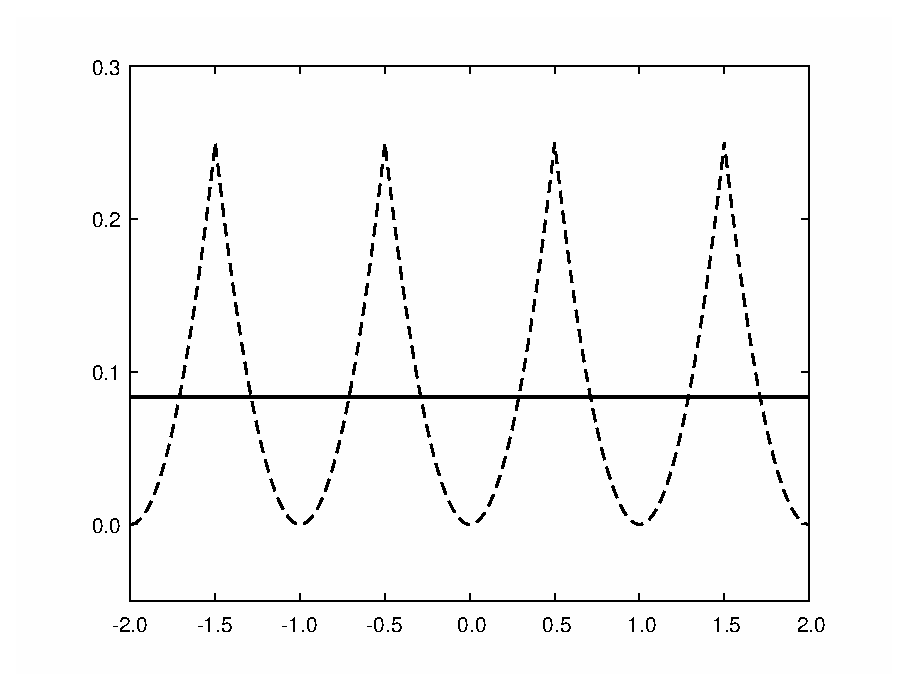
\includegraphics[scale=0.5]{approx1_000}
\subcaption{$v_0(t)$}
\end{subfigure}
\begin{subfigure}{0.48\textwidth}
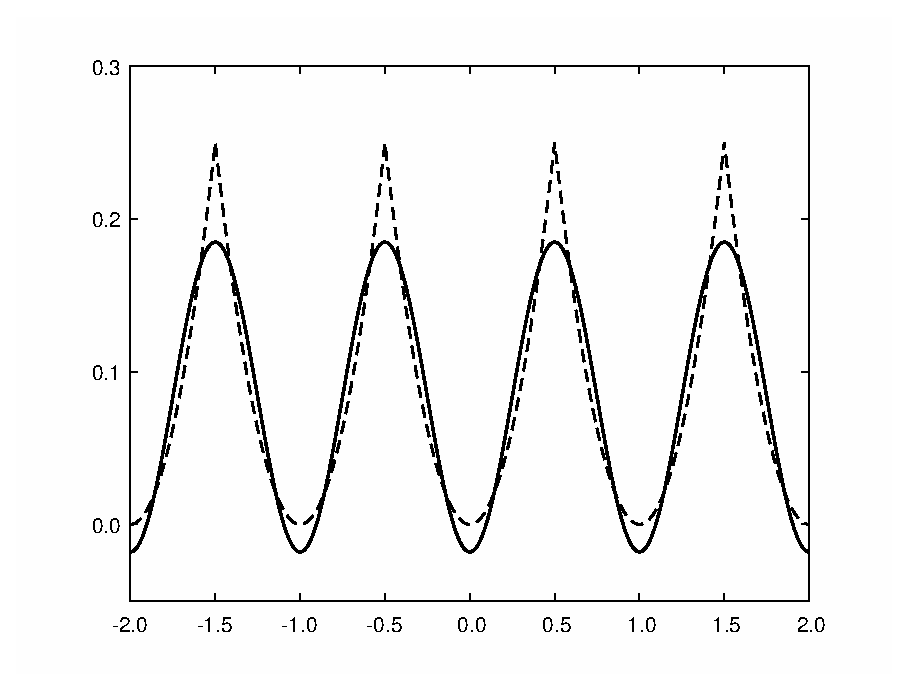
\includegraphics[scale=0.5]{approx1_001}
\subcaption{$v_1(t)$}
\end{subfigure}
\begin{subfigure}{0.48\textwidth}
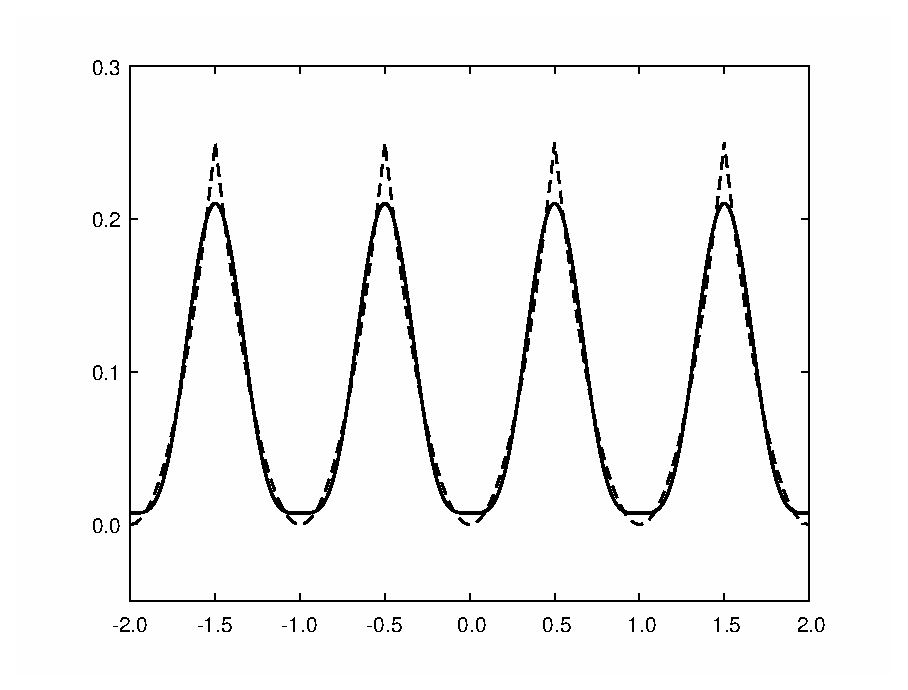
\includegraphics[scale=0.5]{approx1_002}
\subcaption{$v_2(t)$}
\end{subfigure}
\begin{subfigure}{0.48\textwidth}
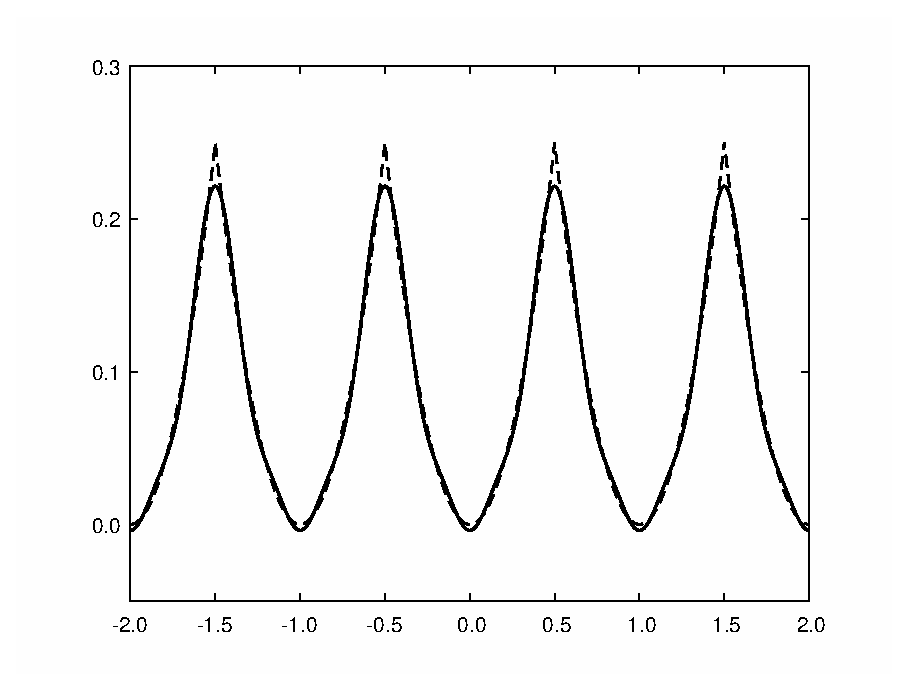
\includegraphics[scale=0.5]{approx1_003}
\subcaption{$v_3(t)$}
\end{subfigure}
\begin{subfigure}{0.48\textwidth}
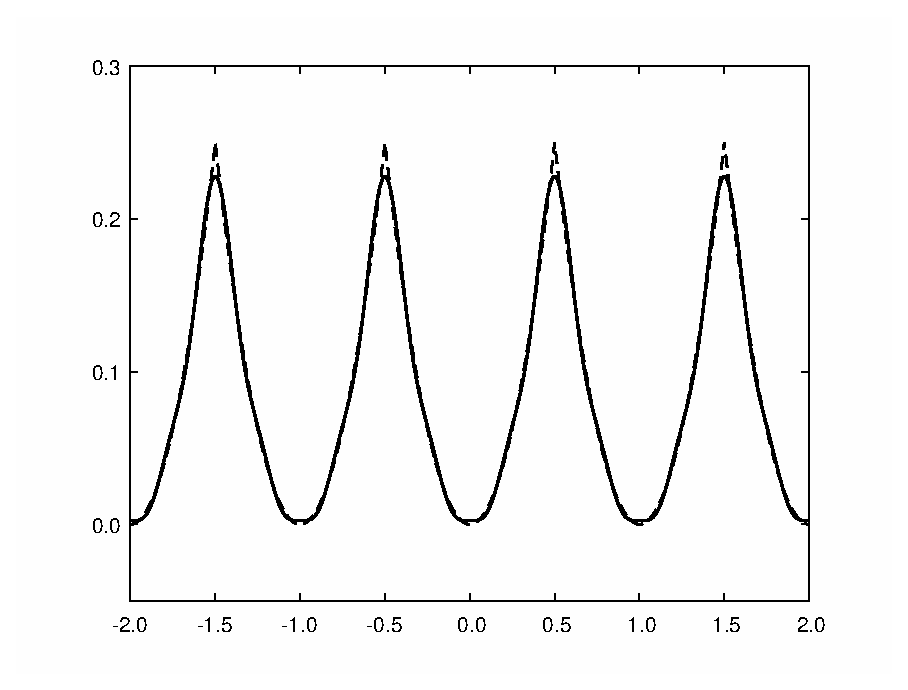
\includegraphics[scale=0.5]{approx1_004}
\subcaption{$v_4(t)$}
\end{subfigure}
\begin{subfigure}{0.48\textwidth}
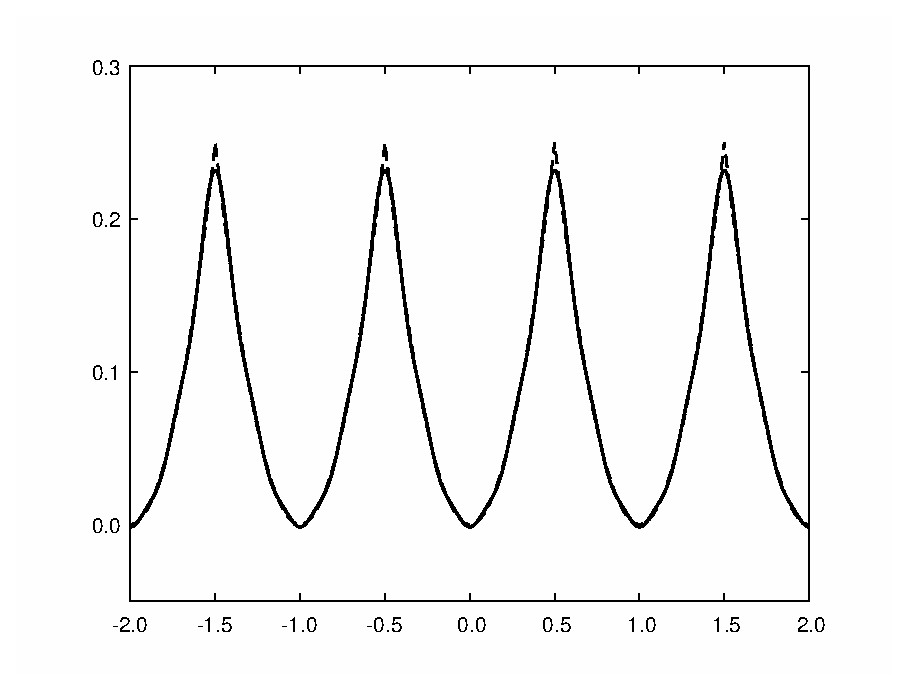
\includegraphics[scale=0.5]{approx1_005}
\subcaption{$v_5(t)$}
\end{subfigure}
\caption{\label{fig:figapprox1}Approksimation til $t^2$ signal.}
\end{figure}

Som endnu et eksempel kan betragtes firkantsignalet i figur~\ref{fig:squareperiodic}b). I dette tilfælde fås koefficienterne ($k\ge{}0$)
\begin{equation}
A_{k} = \frac{4\cdot\sin\left(\frac{\pi\cdot{}k}{2}\right)}{\pi\cdot{}k}
\qquad{}\textrm{samt}
\qquad{}B_{k} = 0.
\end{equation}
Bemærk, at i dette tilfælde er $A_k=0$ for lige værdier af $k$.

I figur~\ref{fig:figapprox2} er vist $v_0(t), v_1(t), v_3(t), v_5(t), v_7(t)$ samt $v_{15}(t)$ for firkantpulsen.
\begin{figure}[htbp]
\centering
\begin{subfigure}{0.48\textwidth}
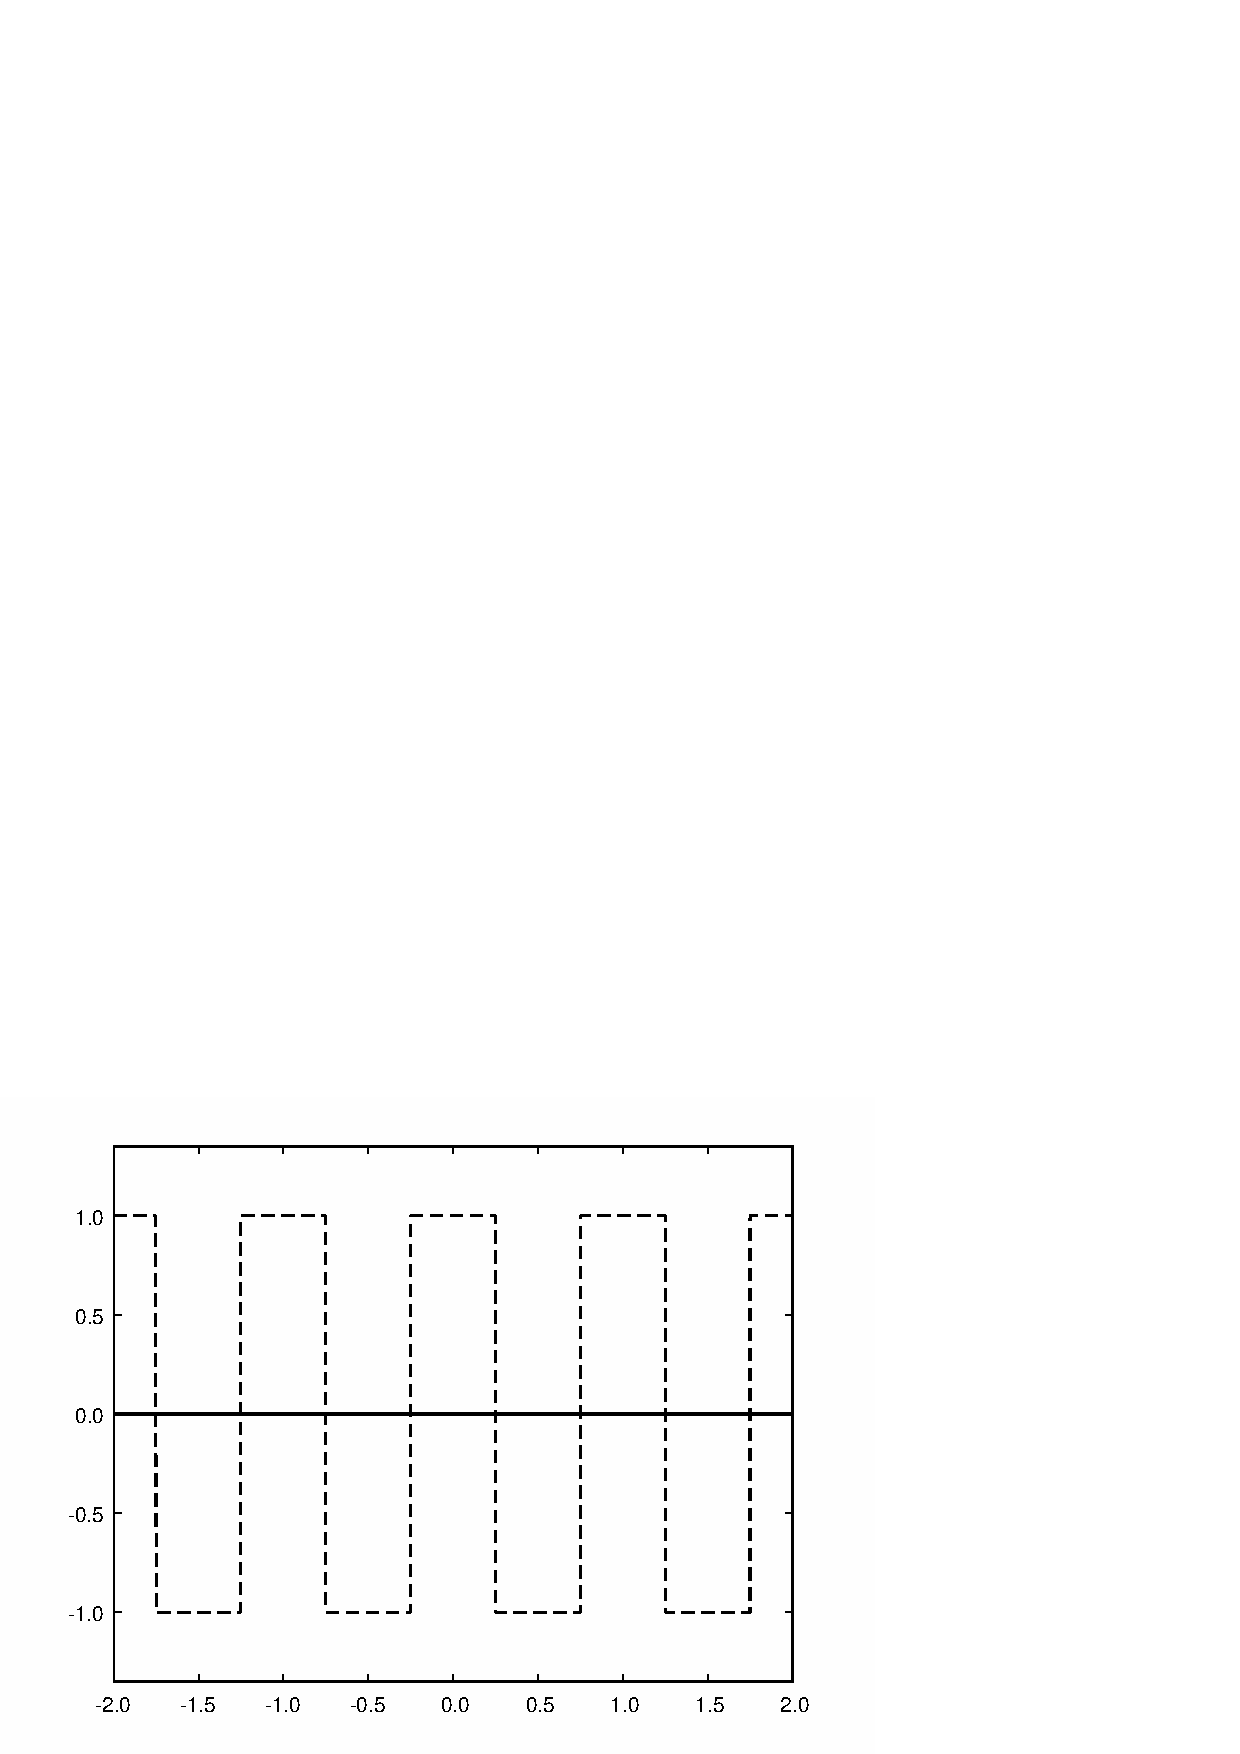
\includegraphics[scale=0.5]{approx2_000}
\subcaption{$v_0(t)$}
\end{subfigure}
\begin{subfigure}{0.48\textwidth}
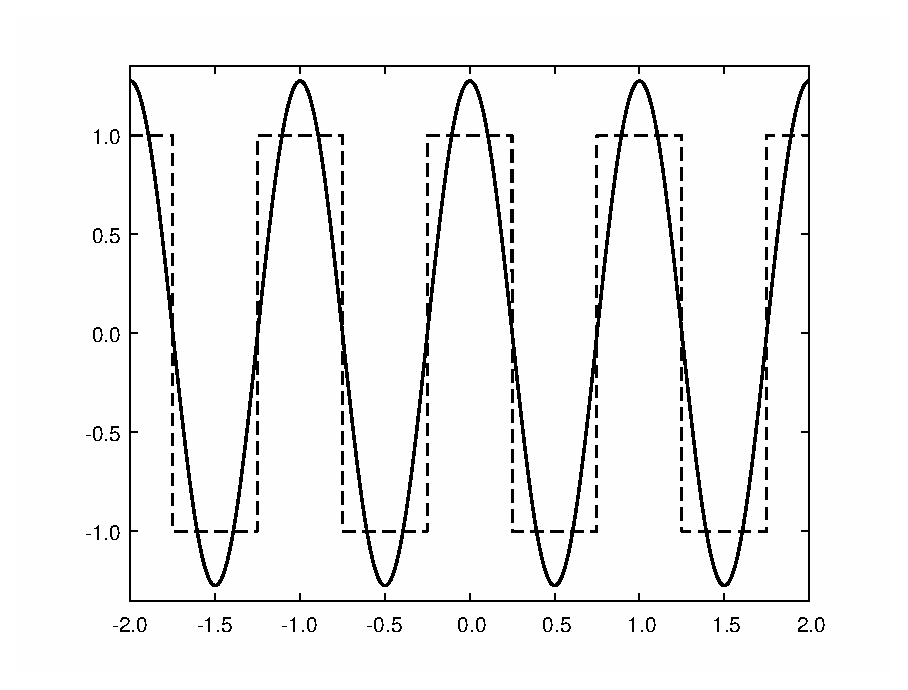
\includegraphics[scale=0.5]{approx2_001}
\subcaption{$v_1(t)$}
\end{subfigure}
\begin{subfigure}{0.48\textwidth}
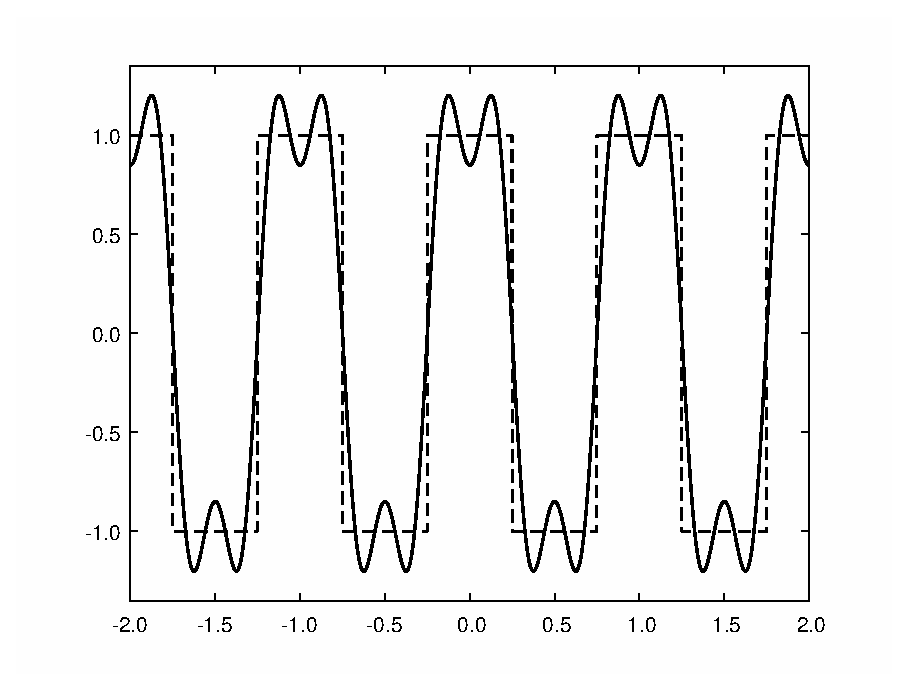
\includegraphics[scale=0.5]{approx2_003}
\subcaption{$v_3(t)$}
\end{subfigure}
\begin{subfigure}{0.48\textwidth}
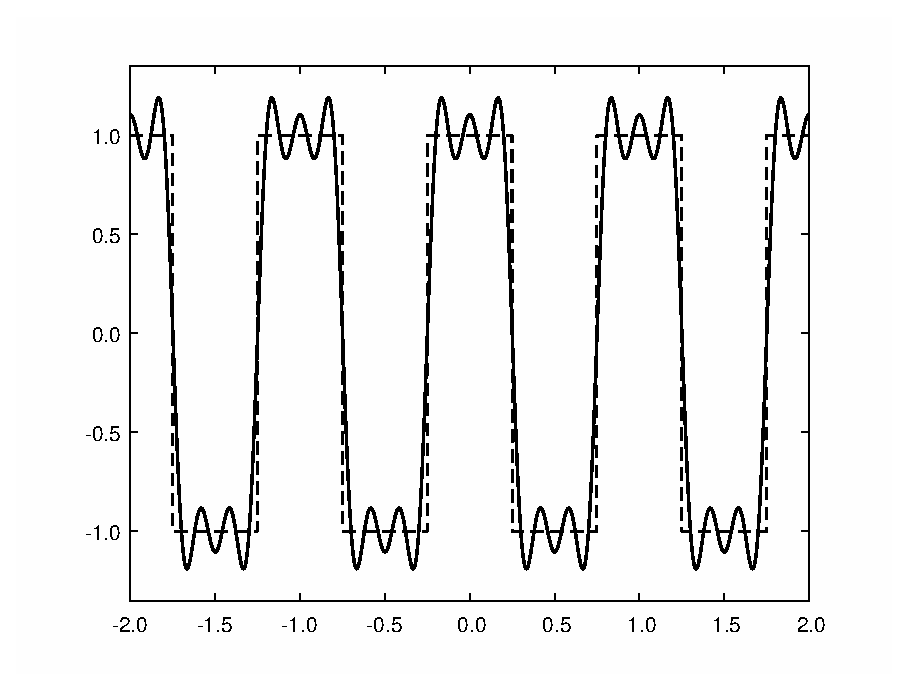
\includegraphics[scale=0.5]{approx2_005}
\subcaption{$v_5(t)$}
\end{subfigure}
\begin{subfigure}{0.48\textwidth}
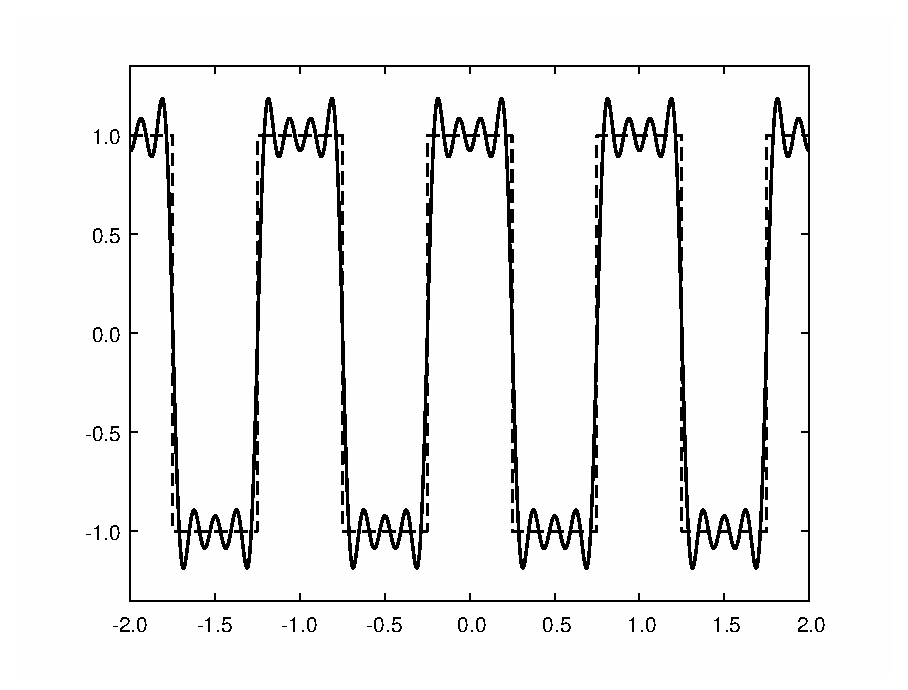
\includegraphics[scale=0.5]{approx2_007}
\subcaption{$v_7(t)$}
\end{subfigure}
\begin{subfigure}{0.48\textwidth}
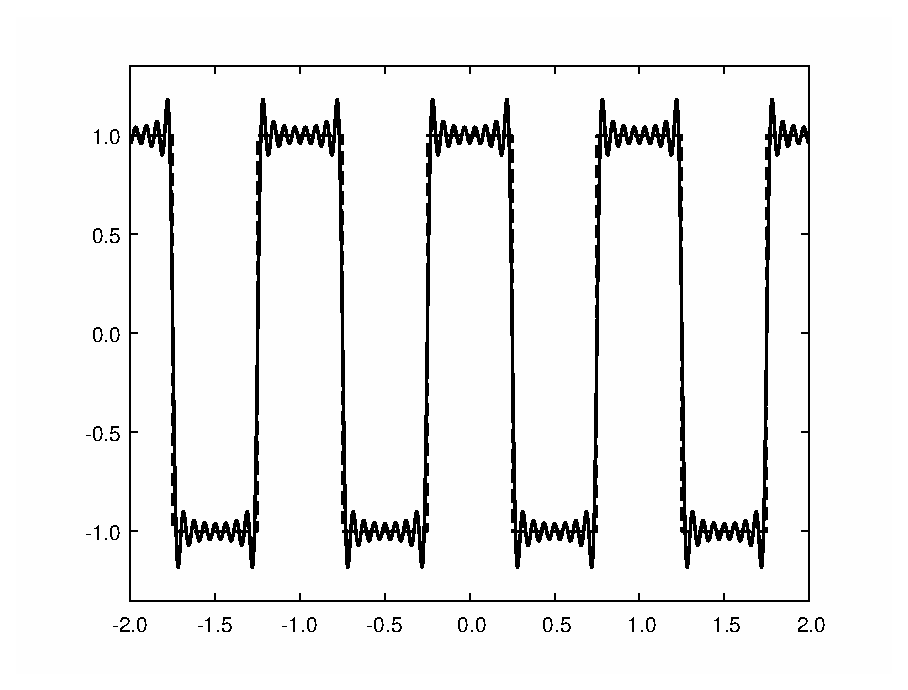
\includegraphics[scale=0.5]{approx2_015}
\subcaption{$v_{15}(t)$}
\end{subfigure}
\caption{\label{fig:figapprox2}Approksimation til firkantsignal.}
\end{figure}

\section{Kompleks repræsentation}
Sætning 3 viser, hvordan en periodisk funktion kan opbygges som en linearkombination af $\cos()$ og $\sin()$ funktioner, og at man for hver frekvens skal kende både $A_k$ og $B_k$ koefficienterne. I praksis foretrækkes en kompleks notation, hvor $\cos()$- og $\sin()$-funktionerne erstattes af komplekse eksponentialfunktioner. Fra kursus 01005 huskes (forhåbentlig) relationerne:
\begin{align}
\cos(x) &= \frac{e^{i\cdot{}x}+e^{-i\cdot{}x}}{2}\\
\sin(x) &= \frac{e^{i\cdot{}x}-e^{-i\cdot{}x}}{2i}\\
e^{ix}  &= \cos(x) + i\cdot\sin(x)\\
e^{-ix} &= \cos(x) - i\cdot\sin(x)
\end{align}

\noindent{}Jf. sætning 3 kan et periodisk signal skrives som et konstant bidrag plus en (evt. uendelig) sum af led af formen (for $k>0$):
\begin{equation}
A_k\cdot\cos(2\pi\cdot{}k\cdot{}f_0\cdot{}t)+B_k\cdot\sin(2\pi\cdot{}k\cdot{}f_0\cdot{}t)
\end{equation}
\noindent{}som kan omskrives på følgende måde:
\begin{multline}
A_k\cdot\cos(2\pi\cdot{}k\cdot{}f_0\cdot{}t)+B_k\cdot\sin(2\pi\cdot{}k\cdot{}f_0\cdot{}t) = \\
A_k\cdot\left(\frac{e^{i2\pi\cdot{}k\cdot{}f_0\cdot{}t}+e^{-i2\pi\cdot{}k\cdot{}f_0\cdot{}t}}{2}\right)+B_k\cdot\left(\frac{e^{i2\pi\cdot{}k\cdot{}f_0\cdot{}t}-e^{-i2\pi\cdot{}k\cdot{}f_0\cdot{}t}}{2i}\right)\\		
\left(\frac{A_k}{2}-i\frac{B_k}{2}\right)e^{i2\pi\cdot{}k\cdot{}f_0\cdot{}t}+\left(\frac{A_k}{2}+i\frac{B_k}{2}\right)e^{-i2\pi\cdot{}k\cdot{}f_0\cdot{}t}
\end{multline}

\noindent{}Introduceres (igen for $k>0$) $V_k=\frac{A_k}{2}-i\frac{B_k}{2}$ fås derfor
\begin{equation}
A_k\cdot\cos(2\pi\cdot{}k\cdot{}f_0\cdot{}t)+B_k\cdot\sin(2\pi\cdot{}k\cdot{}f_0\cdot{}t) = V_{k}e^{i2\pi\cdot{}k\cdot{}f_0\cdot{}t}+\overline{V_{k}}e^{-i2\pi\cdot{}k\cdot{}f_0\cdot{}t}
\end{equation}
\noindent{}hvor $\overline{X}$ betegner den kompleks konjugerede værdi af $X$. For $k=0$ indføres blot $V_0=A_0$. Bemærk, at der ikke er nogen imaginærdel på $V_0$, da $B_0$ pr. definition er lig 0. Hvis man endvidere indfører $V_{-k}=\overline{V_{k}}$ fås:
\begin{equation}
A_k\cdot\cos(2\pi\cdot{}k\cdot{}f_0\cdot{}t)+B_k\cdot\sin(2\pi\cdot{}k\cdot{}f_0\cdot{}t) = V_{k}e^{i2\pi\cdot{}k\cdot{}f_0\cdot{}t}+V_{-k}e^{-i2\pi\cdot{}k\cdot{}f_0\cdot{}t}
\end{equation}

\noindent{}Med den komplekse eksponentialfunktion og de komplekse koefficienter, $V_k$, kan sætning 3 nu omformuleres til:

\vspace{\baselineskip}\fbox{\parbox{0.9\textwidth}{\textbf{Sætning 4:} Enhver kontinuert periodisk funktion, $v(t)$ med perioden $P$ (og dermed grundfrekvensen $f_0$) kan beskrives ved:
\begin{equation}\label{eq:periodic8}
v(t)=V_0 + \sum_{k=1}^{\infty} \left\lbrace{}V_{k}e^{i2\pi\cdot{}k\cdot{}f_0\cdot{}t}+V_{-k}e^{i2\pi\cdot{}k\cdot{}f_0\cdot{}t}\right\rbrace=\sum_{k=-\infty}^{\infty}V_{k}e^{i2\pi\cdot{}k\cdot{}f_0\cdot{}t}
\end{equation}}}\vspace{\baselineskip}

\noindent{}Sidstnævnte udtryk er den såkaldte \emph{Fourierrække} (efter Jean-Baptiste Joseph Fourier) (figur~\ref{fig:jbjfourier}) for et periodisk signal, og $V_k$-værdierne kaldes signalets \emph{Fourierkoefficienter}.
\begin{figure}[htbp]
\centering
\scalebox{0.333}{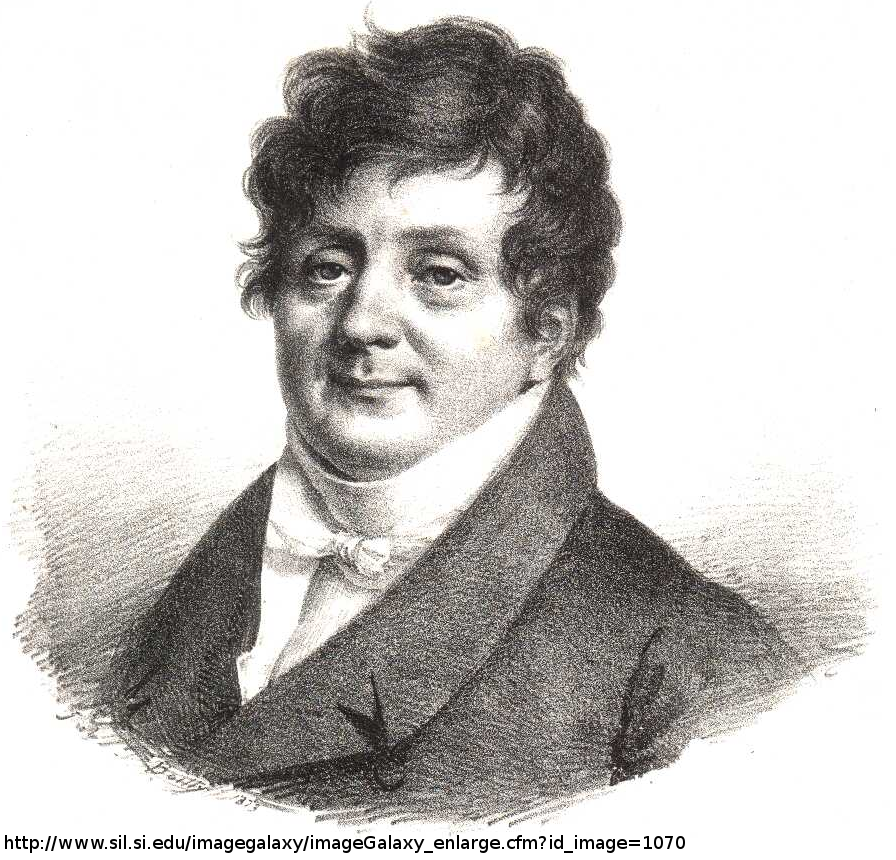
\includegraphics{jbjfourier_v2}}
\label{fig:jbjfourier}
\caption{\label{fig:jbjfourier}Jean-Baptiste Joseph Fourier (1768-1830).}
\end{figure}
% % Kilde til billede af Fourier: 
% % http://www.sil.si.edu/imagegalaxy/imageGalaxy_enlarge.cfm?id_image=1070
% % Burde nok inkluderes på en eller anden måde...

Dvs. et vilkårligt periodisk signal kan beskrives både ved en tidsfunktion (dvs. $v(t)$) men også ved en Fourierrække. Det er vigtigt at forstå, at \emph{begge} beskrivelser indeholder den samme fuldstændige information om signalet. Det er naturligvis det samme signal der er tale om, uanset hvilken af beskrivelserne man benytter; der er blot tale om forskellige måder at beskrive det på.

Beskrivelsen ved en funktion af tiden, $t$ siges at være i tidsdomænet, mens beskrivelsen ved Fourierkoefficienter siges at være i frekvensdomæneet, fordi Fourierkoefficienterne beskriver, hvor meget de enkelte frekvenser ''vægter'' i det endelige signal.



\section{Bestemmelse af Fourierkoefficienter}
Fourierkoefficienter, $V_k$ for $k>0$ kan bestemmes ud fra relationen $V_k=\frac{A_k}{2}-i\frac{B_k}{2}$ og formlerne~(\ref{eq:akoeff}) og (\ref{eq:bkoeff}).
\begin{align}
&V_k = \frac{A_k}{2}-i\frac{B_k}{2} = \nonumber\\
&\frac{1}{P}\cdot\int\limits_{-\frac{P}{2}}^{\frac{P}{2}}v(t)\cdot\cos(2\pi\cdot{}k\cdot{}f_{0}\cdot{}t)\;dt -  \frac{i}{P}\cdot\int\limits_{-\frac{P}{2}}^{\frac{P}{2}}v(t)\cdot\sin(2\pi\cdot{}k\cdot{}f_{0}\cdot{}t)\;dt = \nonumber\\
&\frac{1}{P}\cdot\int\limits_{-\frac{P}{2}}^{\frac{P}{2}}v(t)\cdot\left(\cos(2\pi\cdot{}k\cdot{}f_{0}\cdot{}t) - i\sin(2\pi\cdot{}k\cdot{}f_{0}\cdot{}t)\right)\;dt = \nonumber\\
&\frac{1}{P}\cdot\int\limits_{-\frac{P}{2}}^{\frac{P}{2}}v(t)\cdot{}e^{-2\pi\cdot{}k\cdot{}f_0\cdot{}t}\;dt\label{eq:vposkoeff}
\end{align}

\noindent{}Fourierkoefficienterne, $V_{-k}$ for $k>0$ kan bestemmes på samme måde:
\begin{align}
&V_{-k} = \overline{V_k} = \frac{A_k}{2}+i\frac{B_k}{2} = \nonumber\\
&\frac{1}{P}\cdot\int\limits_{-\frac{P}{2}}^{\frac{P}{2}}v(t)\cdot\cos(2\pi\cdot{}k\cdot{}f_{0}\cdot{}t)\;dt +  \frac{i}{P}\cdot\int\limits_{-\frac{P}{2}}^{\frac{P}{2}}v(t)\cdot\sin(2\pi\cdot{}k\cdot{}f_{0}\cdot{}t)\;dt = \nonumber\\
&\frac{1}{P}\cdot\int\limits_{-\frac{P}{2}}^{\frac{P}{2}}v(t)\cdot\left(\cos(2\pi\cdot{}k\cdot{}f_{0}\cdot{}t) + i\sin(2\pi\cdot{}k\cdot{}f_{0}\cdot{}t)\right)\;dt = \nonumber\\
&\frac{1}{P}\cdot\int\limits_{-\frac{P}{2}}^{\frac{P}{2}}v(t)\cdot\left(\cos(2\pi\cdot{}k\cdot{}f_{0}\cdot{}t) - i\sin(2\pi\cdot{}(-k)\cdot{}f_{0}\cdot{}t)\right)\;dt = \nonumber\\
&\frac{1}{P}\cdot\int\limits_{-\frac{P}{2}}^{\frac{P}{2}}v(t)\cdot{}e^{-2\pi\cdot{}(-k)\cdot{}f_0\cdot{}t}\;dt\label{eq:vnegkoeff}
\end{align}

\noindent{}Endelig for $k=0$ fås, da $V_0=A_0$,
\begin{gather}
V_0 = A_0 = \frac{1}{P}\cdot{}\int\limits_{-\frac{P}{2}}^{\frac{P}{2}}v(t)\;dt = \frac{1}{P}\cdot{}\int\limits_{-\frac{P}{2}}^{\frac{P}{2}}v(t)\cdot{}e^{-2\pi\cdot{}0\cdot{}f_0\cdot{}t}\;dt\label{eq:vzerokoeff}
\end{gather}
\noindent{}da $e^{-2\pi\cdot{}0\cdot{}f_0\cdot{}t}=1$. 

Bemærk ligheden mellem formlerne~(\ref{eq:vposkoeff}), (\ref{eq:vnegkoeff}) og (\ref{eq:vzerokoeff}), specielt omkring fortegnet for $k$ i argumentet til eksponentialfunktionen. Herved ses at disse formler kan ''slås sammen'', dvs. at \emph{samtlige}\footnote{Dvs. både for $k<0$, $k=0$ og $k>0$.} Fourierkoefficienter, $V_k$ ($k\in\mathbb{Z}$), kan findes ud fra formel~(\ref{eq:vallkoeff}):
\begin{equation}
V_k = \frac{1}{P}\cdot\int\limits_{-\frac{P}{2}}^{\frac{P}{2}}v(t)\cdot{}e^{-2\pi\cdot{}k\cdot{}f_0\cdot{}t}\;dt\label{eq:vallkoeff}
\end{equation}

\noindent{}Dvs. vi kan nu endelig formulere den gennemgående sætning som:

\vspace{\baselineskip}\fbox{\parbox{0.9\textwidth}{\textbf{Sætning 5:} Enhver kontinuert periodisk funktion, $v(t)$, med perioden $P$ (og dermed grundfrekvensen $f_0$) kan beskrives ved Fourierrækken:
\begin{equation}\label{eq:ifourier}
v(t)=\sum_{k=-\infty}^{\infty}V_{k}e^{i2\pi\cdot{}k\cdot{}f_0\cdot{}t}
\end{equation}
\noindent{}hvor Fourierkoefficienterne, $V_k$, kan udregnes som
\begin{equation}\label{eq:fourier}
V_k = \frac{1}{P}\cdot\int\limits_{-\frac{P}{2}}^{\frac{P}{2}}v(t)\cdot{}e^{-2\pi\cdot{}k\cdot{}f_0\cdot{}t}\;dt
\end{equation}
}}\vspace{\baselineskip}

\noindent{}Dette er et fundamentalt og vigtigt resultat i forbindelse med analyse af signaler og kommunikationssystemer, da det viser, hvordan man skifter repræsentation af et signal mellem tids- og frekvensdomænet. Der gælder nemlig:
\begin{itemize}
%
\item Hvis man kender signalets Fourierkoefficienter, $V_k$, (dvs. man har en beskrivelse af signalet i frekvensdomænet) kan man via formel~(\ref{eq:ifourier}) udregne signalets tidsfunktion, dvs. signalet i tidsdomænet.
%
\item Hvis man kender signalet som funktion af tiden, $t$, (dvs. man kender signalet i tidsdomænet) kan man via formel~(\ref{eq:fourier}) udregne dets Fourierkoefficienter, dvs. bestemme signalet i frekvensdomænet.
%
\end{itemize}
\noindent{}Dvs. vi har fuld viden om et periodisk signal, hvis bare vi kender enten beskrivelsen i tidsdomænet (dvs. via funktionen $v(t)$) eller Fourierkoefficienterne for signalet (dvs. signalets $V_k$-værdier), og vi kan altid skifte mellem de to domæner ved hjælp af formlerne~(\ref{eq:ifourier}) og~(\ref{eq:fourier}).


\end{document}